\documentclass[10pt,a4paper]{article}
\usepackage{fullpage}
\usepackage[utf8]{inputenc}
\usepackage[english]{babel}
\usepackage[hidelinks]{hyperref}
\usepackage{amsmath}
\usepackage{amsfonts}
\usepackage{float}
\usepackage{subcaption}
\usepackage{tikz}
\usetikzlibrary{colorbrewer}
\usepackage{pgfplots}
\usepackage{pgfplotstable}
\pgfplotsset{compat=newest}
\usepgfplotslibrary{colorbrewer}
\usepgfplotslibrary{groupplots}
\usepgfplotslibrary{units}
% \usepgfplotslibrary{external}
% \tikzexternalize

\usepackage{mathrm}
\usepackage{mat-vec}

\definecolor{brewergreylight}{RGB}{224,224,224}
\definecolor{brewergrey}{RGB}{99,99,99}
\definecolor{brewerred}{RGB}{227,74,51}
\definecolor{brewerblue}{RGB}{33,113,181}
\definecolor{brewergreen}{RGB}{49,163,84}
\definecolor{brewergreendark}{RGB}{152,78,163}
\definecolor{breweryellow}{RGB}{27,120,55}

\listfiles

\begin{document}
\title{IGA of a Photocathode}
\date{}
\author{}
\maketitle

\tableofcontents

% \section{60 kV Geometry}
% \subsection{Geometry}
The $60$ kV geometry was derived from the technical drawings in \cite{espig}. Some simplifications were made especially regarding the inner part of the electrode, such that the geometry may be modeled as being rotationally symmetric. The dimensions of the electrode, puck, puck elevator, vacuum chamber and insulator were derived from Figure A.1, A.2, A.3, A.4 and A.6 in \cite{espig} respectively. The geometry of the vacuum chamber was also simplified to reduce the computational domain and the reduced insulator geometry is in part based on the drawing in Figure 5.7 of the thesis.
The boundary conditions were retrieved from Table 5.1 in \cite{espig} and the relative permittivity of the insulator was taken from an existing CST model to be $9.4$.

The geometry is depicted in fig.~\ref{fig:geometry} and a technical drawing of the actual geometry is given in fig.~\ref{fig:cad_geometry} for comparison. The numbers in the simplified geometry refer to the individual patches in the context of IGA. The patch boundaries are indicated by the black lines. The red lines represent homogeneous Dirichlet boundary conditions, the blue lines inhomogeneous Dirichlet boundary conditions with a value of $-60\ \mathrm{kV}$ and the green lines indicate homogeneous Neumann boundaries.
According to the technical drawings patch $10$ as well as parts of patches $7$ and $8$ are modeled as insulator material.

\begin{center}
\begin{figure}[H]
  \begin{tikzpicture}
\begin{axis}[
   scale only axis = true,
   width = 0.9\textwidth,
  axis equal,
  try min ticks=4,
  max space between ticks=1000pt,
  enlargelimits=true,
  colormap/Greens,
  point meta min = 0,
  point meta max = 2,
  x unit=m,
  y unit=m]

  \addplot[surf, shader=interp] table[point meta=\thisrow{c}]{figures/200kV/geometry/geometry_1.dat};

  \addplot[surf, shader=interp] table[point meta=\thisrow{c}]{figures/200kV/geometry/geometry_2.dat};

  \addplot[surf, shader=interp] table[point meta=\thisrow{c}]{figures/200kV/geometry/geometry_3.dat};

  \addplot[surf, shader=interp] table[point meta=\thisrow{c}]{figures/200kV/geometry/geometry_4.dat};

  \addplot[surf, shader=interp] table[point meta=\thisrow{c}]{figures/200kV/geometry/geometry_5.dat};

  \addplot[surf, shader=interp] table[point meta=\thisrow{c}]{figures/200kV/geometry/geometry_6.dat};

  \addplot[surf, shader=interp] table[point meta=\thisrow{c}]{figures/200kV/geometry/geometry_7.dat};

  \addplot[surf, shader=interp] table[point meta=\thisrow{c}]{figures/200kV/geometry/geometry_8.dat};

  \addplot[surf, shader=interp] table[point meta=\thisrow{c}]{figures/200kV/geometry/geometry_9.dat};

  \addplot[surf, shader=interp] table[point meta=\thisrow{c}]{figures/200kV/geometry/geometry_10.dat};

  \addplot[surf, shader=interp] table[point meta=\thisrow{c}]{figures/200kV/geometry/geometry_11.dat};

  \addplot[surf, shader=interp] table[point meta=\thisrow{c}]{figures/200kV/geometry/geometry_12.dat};

  \addplot[surf, shader=interp] table[point meta=\thisrow{c}]{figures/200kV/geometry/geometry_13.dat};

  \addplot[surf, shader=interp, colormap/Reds, point meta min = 0, point meta max = 1] table[point meta=\thisrow{c}]{figures/200kV/geometry/geometry_13.dat};

  \addplot[surf, shader=interp] table[point meta=\thisrow{c}]{figures/200kV/geometry/geometry_14.dat};

  \addplot[surf, shader=interp] table[point meta=\thisrow{c}]{figures/200kV/geometry/geometry_15.dat};

  \addplot[surf, shader=interp, colormap/Reds, point meta min = 0, point meta max = 1] table[point meta=\thisrow{c}]{figures/200kV/geometry/geometry_16.dat};

  \addplot[surf, shader=interp, colormap/Reds, point meta min = 0, point meta max = 1] table[point meta=\thisrow{c}]{figures/200kV/geometry/geometry_17.dat};

  \addplot[surf, shader=interp] table[point meta=\thisrow{c}]{figures/200kV/geometry/geometry_18.dat};

  \addplot[surf, shader=interp] table[point meta=\thisrow{c}]{figures/200kV/geometry/geometry_19.dat};

  \addplot[surf, shader=interp] table[point meta=\thisrow{c}]{figures/200kV/geometry/geometry_20.dat};

  \addplot[surf, shader=interp] table[point meta=\thisrow{c}]{figures/200kV/geometry/geometry_21.dat};

  \addplot[surf, shader=interp] table[point meta=\thisrow{c}]{figures/200kV/geometry/geometry_22.dat};

  % add patch indices
  \addplot[only marks, point meta=explicit symbolic, color=black, nodes near coords] coordinates{
  (0.28,-0.01) [(1)]
  (0.28,-0.005) [(2)]
  (0.28,0.005) [(3)]
  (0.28,0.015) [(4)]
  (0.28,0.045) [(5)]
  (0.24,0.075) [(6)]
  (0.15,0.075) [(7)]
  (0.085,0.075) [(8)]
  (0.1,0.05) [(9)]
  (0.05,0.065) [(10)]
  (0.1,0.04) [(11)]
  (0.05,0.045) [(12)]
  (0.05,0.03) [(13)]
  (0.03,0.0175) [(14)]
  (0.0075,0.0075) [(15)]
  (0.04,0.007) [(16)]
  (0.0075,0.0025) [(17)]
  (0.075,0.017) [(18)]
  (0.115,0.017) [(19)]
  (0.135,0.015) [(20)]
  (0.155,0.025) [(21)]
  (0.035,-0.005) [(22)]
  };

  % add patch boundaries
  \addplot[color=brewerblue] table{figures/200kV/boundary/boundaries11.dat};
  \addplot[color=brewerred] table{figures/200kV/boundary/boundaries12.dat};
  \addplot[color=black] table{figures/200kV/boundary/boundaries13.dat};
  \addplot[color=brewergrey] table{figures/200kV/boundary/boundaries14.dat};

  \addplot[color=brewerblue] table{figures/200kV/boundary/boundaries21.dat};
  \addplot[color=brewerred] table{figures/200kV/boundary/boundaries22.dat};
  \addplot[color=brewergrey] table{figures/200kV/boundary/boundaries23.dat};
  \addplot[color=brewergrey] table{figures/200kV/boundary/boundaries24.dat};

  \addplot[color=brewerblue] table{figures/200kV/boundary/boundaries31.dat};
  \addplot[color=brewerred] table{figures/200kV/boundary/boundaries32.dat};
  \addplot[color=brewergrey] table{figures/200kV/boundary/boundaries33.dat};
  \addplot[color=brewergrey] table{figures/200kV/boundary/boundaries34.dat};

  \addplot[color=brewerblue] table{figures/200kV/boundary/boundaries41.dat};
  \addplot[color=brewerred] table{figures/200kV/boundary/boundaries42.dat};
  \addplot[color=brewergrey] table{figures/200kV/boundary/boundaries43.dat};
  \addplot[color=brewergrey] table{figures/200kV/boundary/boundaries44.dat};

  \addplot[color=brewerblue] table{figures/200kV/boundary/boundaries51.dat};
  \addplot[color=brewerred] table{figures/200kV/boundary/boundaries52.dat};
  \addplot[color=brewergrey] table{figures/200kV/boundary/boundaries53.dat};
  \addplot[color=brewergrey] table{figures/200kV/boundary/boundaries54.dat};

  \addplot[color=brewerblue] table{figures/200kV/boundary/boundaries61.dat};
  \addplot[color=brewerred] table{figures/200kV/boundary/boundaries62.dat};
  \addplot[color=brewergrey] table{figures/200kV/boundary/boundaries63.dat};
  \addplot[color=brewergrey] table{figures/200kV/boundary/boundaries64.dat};

  \addplot[color=brewerblue] table{figures/200kV/boundary/boundaries71.dat};
  \addplot[color=brewerred] table{figures/200kV/boundary/boundaries72.dat};
  \addplot[color=brewergrey] table{figures/200kV/boundary/boundaries73.dat};
  \addplot[color=brewergrey] table{figures/200kV/boundary/boundaries74.dat};

  \addplot[color=brewergrey] table{figures/200kV/boundary/boundaries81.dat};
  \addplot[color=brewerred] table{figures/200kV/boundary/boundaries82.dat};
  \addplot[color=brewergrey] table{figures/200kV/boundary/boundaries83.dat};
  \addplot[color=brewergrey] table{figures/200kV/boundary/boundaries84.dat};

  \addplot[color=brewergrey] table{figures/200kV/boundary/boundaries91.dat};
  \addplot[color=brewerblue] table{figures/200kV/boundary/boundaries92.dat};
  \addplot[color=brewergrey] table{figures/200kV/boundary/boundaries93.dat};
  \addplot[color=brewergrey] table{figures/200kV/boundary/boundaries94.dat};

  \addplot[color=brewerred] table{figures/200kV/boundary/boundaries101.dat};
  \addplot[color=brewergrey] table{figures/200kV/boundary/boundaries102.dat};
  \addplot[color=brewergrey] table{figures/200kV/boundary/boundaries103.dat};
  \addplot[color=brewergrey] table{figures/200kV/boundary/boundaries104.dat};

  \addplot[color=brewergrey] table{figures/200kV/boundary/boundaries111.dat};
  \addplot[color=brewerblue] table{figures/200kV/boundary/boundaries112.dat};
  \addplot[color=brewerblue] table{figures/200kV/boundary/boundaries113.dat};
  \addplot[color=brewergrey] table{figures/200kV/boundary/boundaries114.dat};

  \addplot[color=brewerred] table{figures/200kV/boundary/boundaries121.dat};
  \addplot[color=brewergrey] table{figures/200kV/boundary/boundaries122.dat};
  \addplot[color=brewergrey] table{figures/200kV/boundary/boundaries123.dat};
  \addplot[color=brewergrey] table{figures/200kV/boundary/boundaries124.dat};

  \addplot[color=brewerred] table{figures/200kV/boundary/boundaries131.dat};
  \addplot[color=brewerblue] table{figures/200kV/boundary/boundaries132.dat};
  \addplot[color=brewergrey] table{figures/200kV/boundary/boundaries133.dat};
  \addplot[color=brewergrey] table{figures/200kV/boundary/boundaries134.dat};

  \addplot[color=brewerred] table{figures/200kV/boundary/boundaries141.dat};
  \addplot[color=brewergrey] table{figures/200kV/boundary/boundaries142.dat};
  \addplot[color=brewergrey] table{figures/200kV/boundary/boundaries143.dat};
  \addplot[color=brewergrey] table{figures/200kV/boundary/boundaries144.dat};

  \addplot[color=brewerred] table{figures/200kV/boundary/boundaries151.dat};
  \addplot[color=brewergrey] table{figures/200kV/boundary/boundaries152.dat};
  \addplot[color=brewergrey] table{figures/200kV/boundary/boundaries153.dat};
  \addplot[color=brewergrey] table{figures/200kV/boundary/boundaries154.dat};

  \addplot[color=brewergrey] table{figures/200kV/boundary/boundaries161.dat};
  \addplot[color=brewerblue] table{figures/200kV/boundary/boundaries162.dat};
  \addplot[color=brewergrey] table{figures/200kV/boundary/boundaries163.dat};
  \addplot[color=brewergrey] table{figures/200kV/boundary/boundaries164.dat};

  \addplot[color=brewerred] table{figures/200kV/boundary/boundaries171.dat};
  \addplot[color=brewergrey] table{figures/200kV/boundary/boundaries172.dat};
  \addplot[color=brewergrey] table{figures/200kV/boundary/boundaries173.dat};
  \addplot[color=brewergrey] table{figures/200kV/boundary/boundaries174.dat};

  \addplot[color=brewergrey] table{figures/200kV/boundary/boundaries181.dat};
  \addplot[color=brewergrey] table{figures/200kV/boundary/boundaries182.dat};
  \addplot[color=brewergrey] table{figures/200kV/boundary/boundaries183.dat};
  \addplot[color=brewerblue] table{figures/200kV/boundary/boundaries184.dat};

  \addplot[color=brewergrey] table{figures/200kV/boundary/boundaries191.dat};
  \addplot[color=brewergrey] table{figures/200kV/boundary/boundaries192.dat};
  \addplot[color=brewerblue] table{figures/200kV/boundary/boundaries193.dat};
  \addplot[color=brewerblue] table{figures/200kV/boundary/boundaries194.dat};

  \addplot[color=brewerblue] table{figures/200kV/boundary/boundaries201.dat};
  \addplot[color=brewergrey] table{figures/200kV/boundary/boundaries202.dat};
  \addplot[color=brewerblue] table{figures/200kV/boundary/boundaries203.dat};
  \addplot[color=brewergrey] table{figures/200kV/boundary/boundaries204.dat};

  \addplot[color=brewerblue] table{figures/200kV/boundary/boundaries211.dat};
  \addplot[color=brewerblue] table{figures/200kV/boundary/boundaries212.dat};
  \addplot[color=brewergrey] table{figures/200kV/boundary/boundaries213.dat};
  \addplot[color=brewerblue] table{figures/200kV/boundary/boundaries214.dat};

  \addplot[color=brewerred] table{figures/200kV/boundary/boundaries221.dat};
  \addplot[color=brewerblue] table{figures/200kV/boundary/boundaries222.dat};
  \addplot[color=black] table{figures/200kV/boundary/boundaries223.dat};
  \addplot[color=brewergrey] table{figures/200kV/boundary/boundaries224.dat};
\end{axis}
\end{tikzpicture}

  \caption{60 kV Photocathode geometry and boundary conditions.}
  \label{fig:geometry}
\end{figure}
\end{center}

\begin{center}
\begin{figure}[H]
  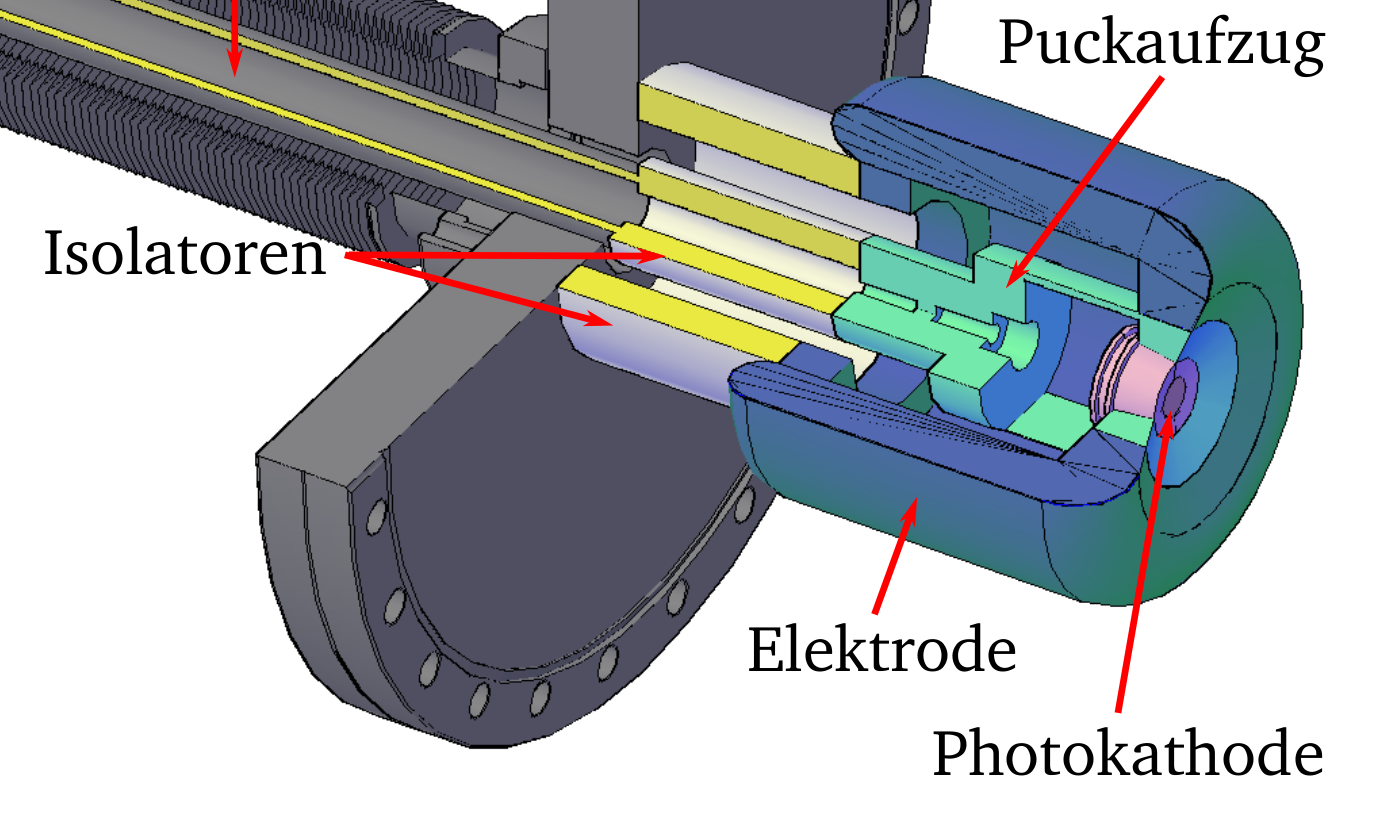
\includegraphics[width=\textwidth]{figures/60kV/geometry}
  \caption{Part of the CAD drawing of the geometry.}
  \label{fig:cad_geometry}
\end{figure}
\end{center}

\subsection{Electrostatic Potential and Electric Field}
\label{sec:potential_field}
The solution for the electrostatic potential is shown in fig.~\ref{fig:potential}. Fig.~\ref{fig:electric_field} depicts the absolute value of the electric field.
Both of the solutions were computed with $p=4$ as the degree of the basis functions and $n_\mathrm{sub}=128$ as the number of elements that each knot vector is uniformly split into.
To give a comparison with the previous simulations fig.~\ref{fig:phd_electric_field} shows the results depicted in the thesis \cite{espig}. It is visible that the solutions are similar with the peak values appearing near the circular parts of the electrode. However the new results indicate that the absolute largest values occur at the back of the electrode and they also show higher field magnitudes in the insulator regions. This is a clear contrast to the previous simulation.
A second comparison can be made with the updated CST model from fig.~\ref{fig:electric_field_wende} from \cite{wende}. The absolute largest field values appear in the same region, however their magnitude is higher.
The bevavior of the field at the triple point is also very similar in that the surrounding magnitudes are very small.

\begin{center}
\begin{figure}[H]
  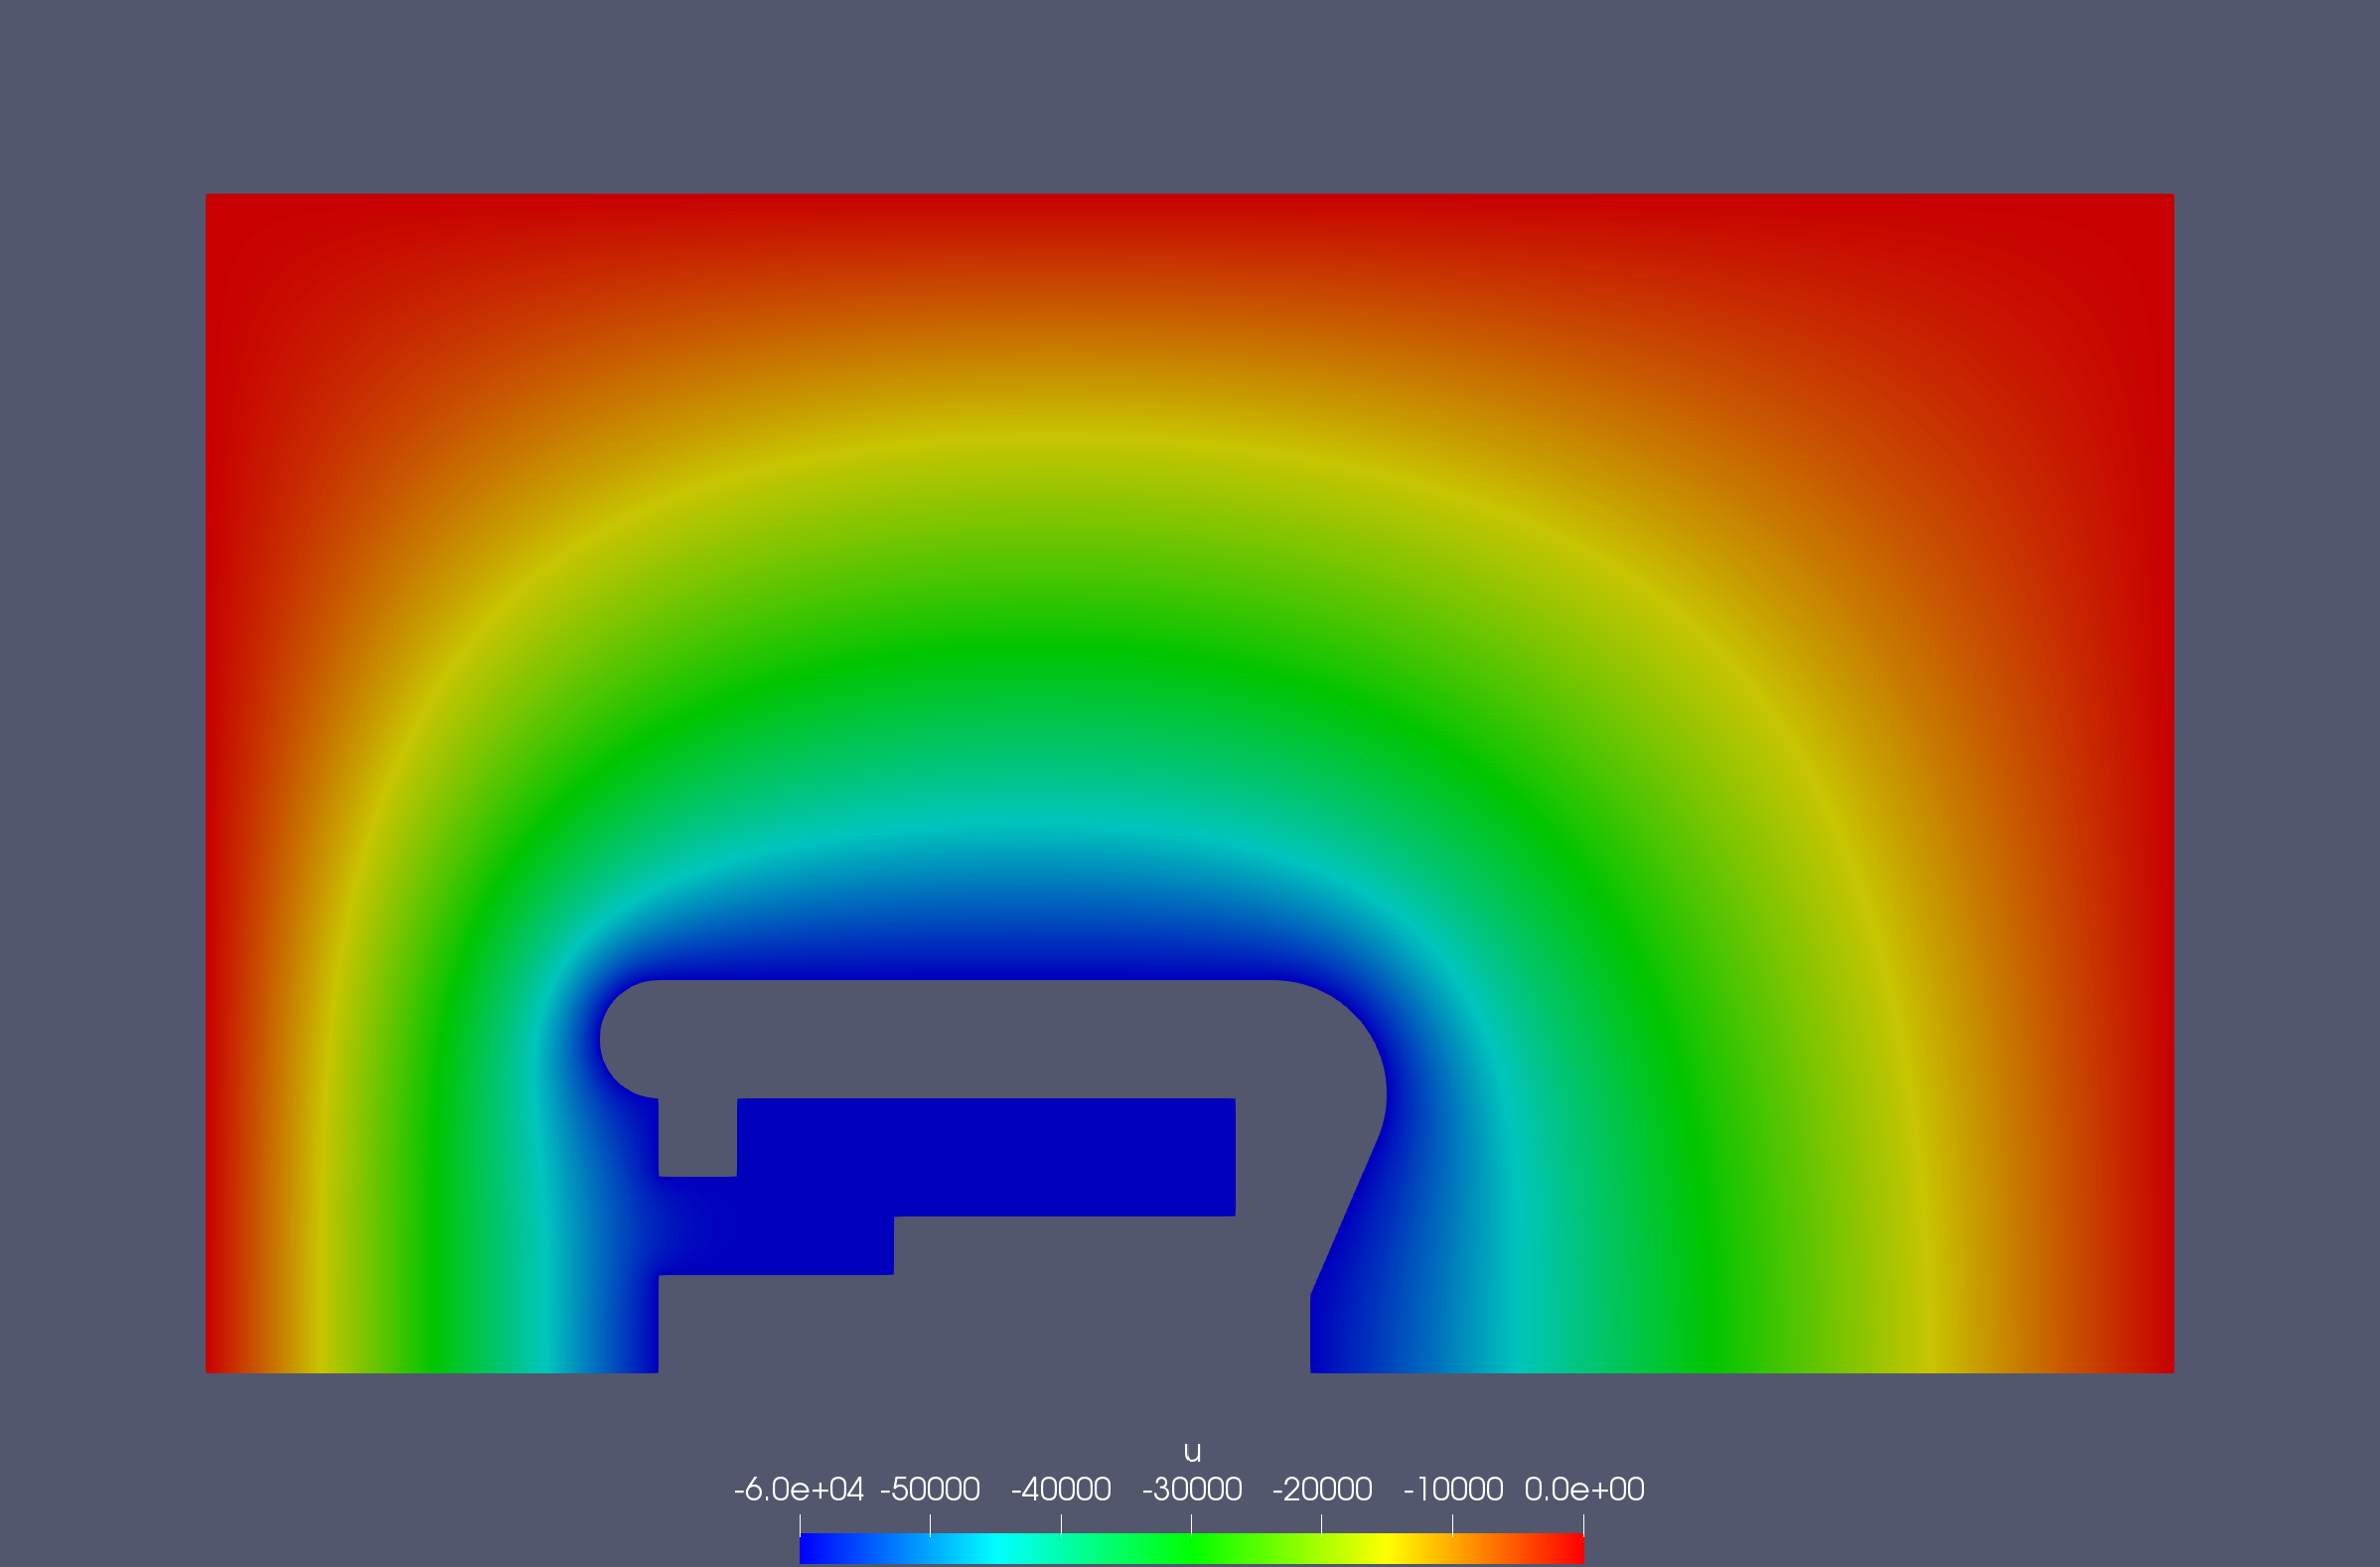
\includegraphics[width=\textwidth]{figures/60kV/potential}
  \caption{Electrostatic potential.}
  \label{fig:potential}
\end{figure}
\end{center}

\begin{center}
\begin{figure}[H]
  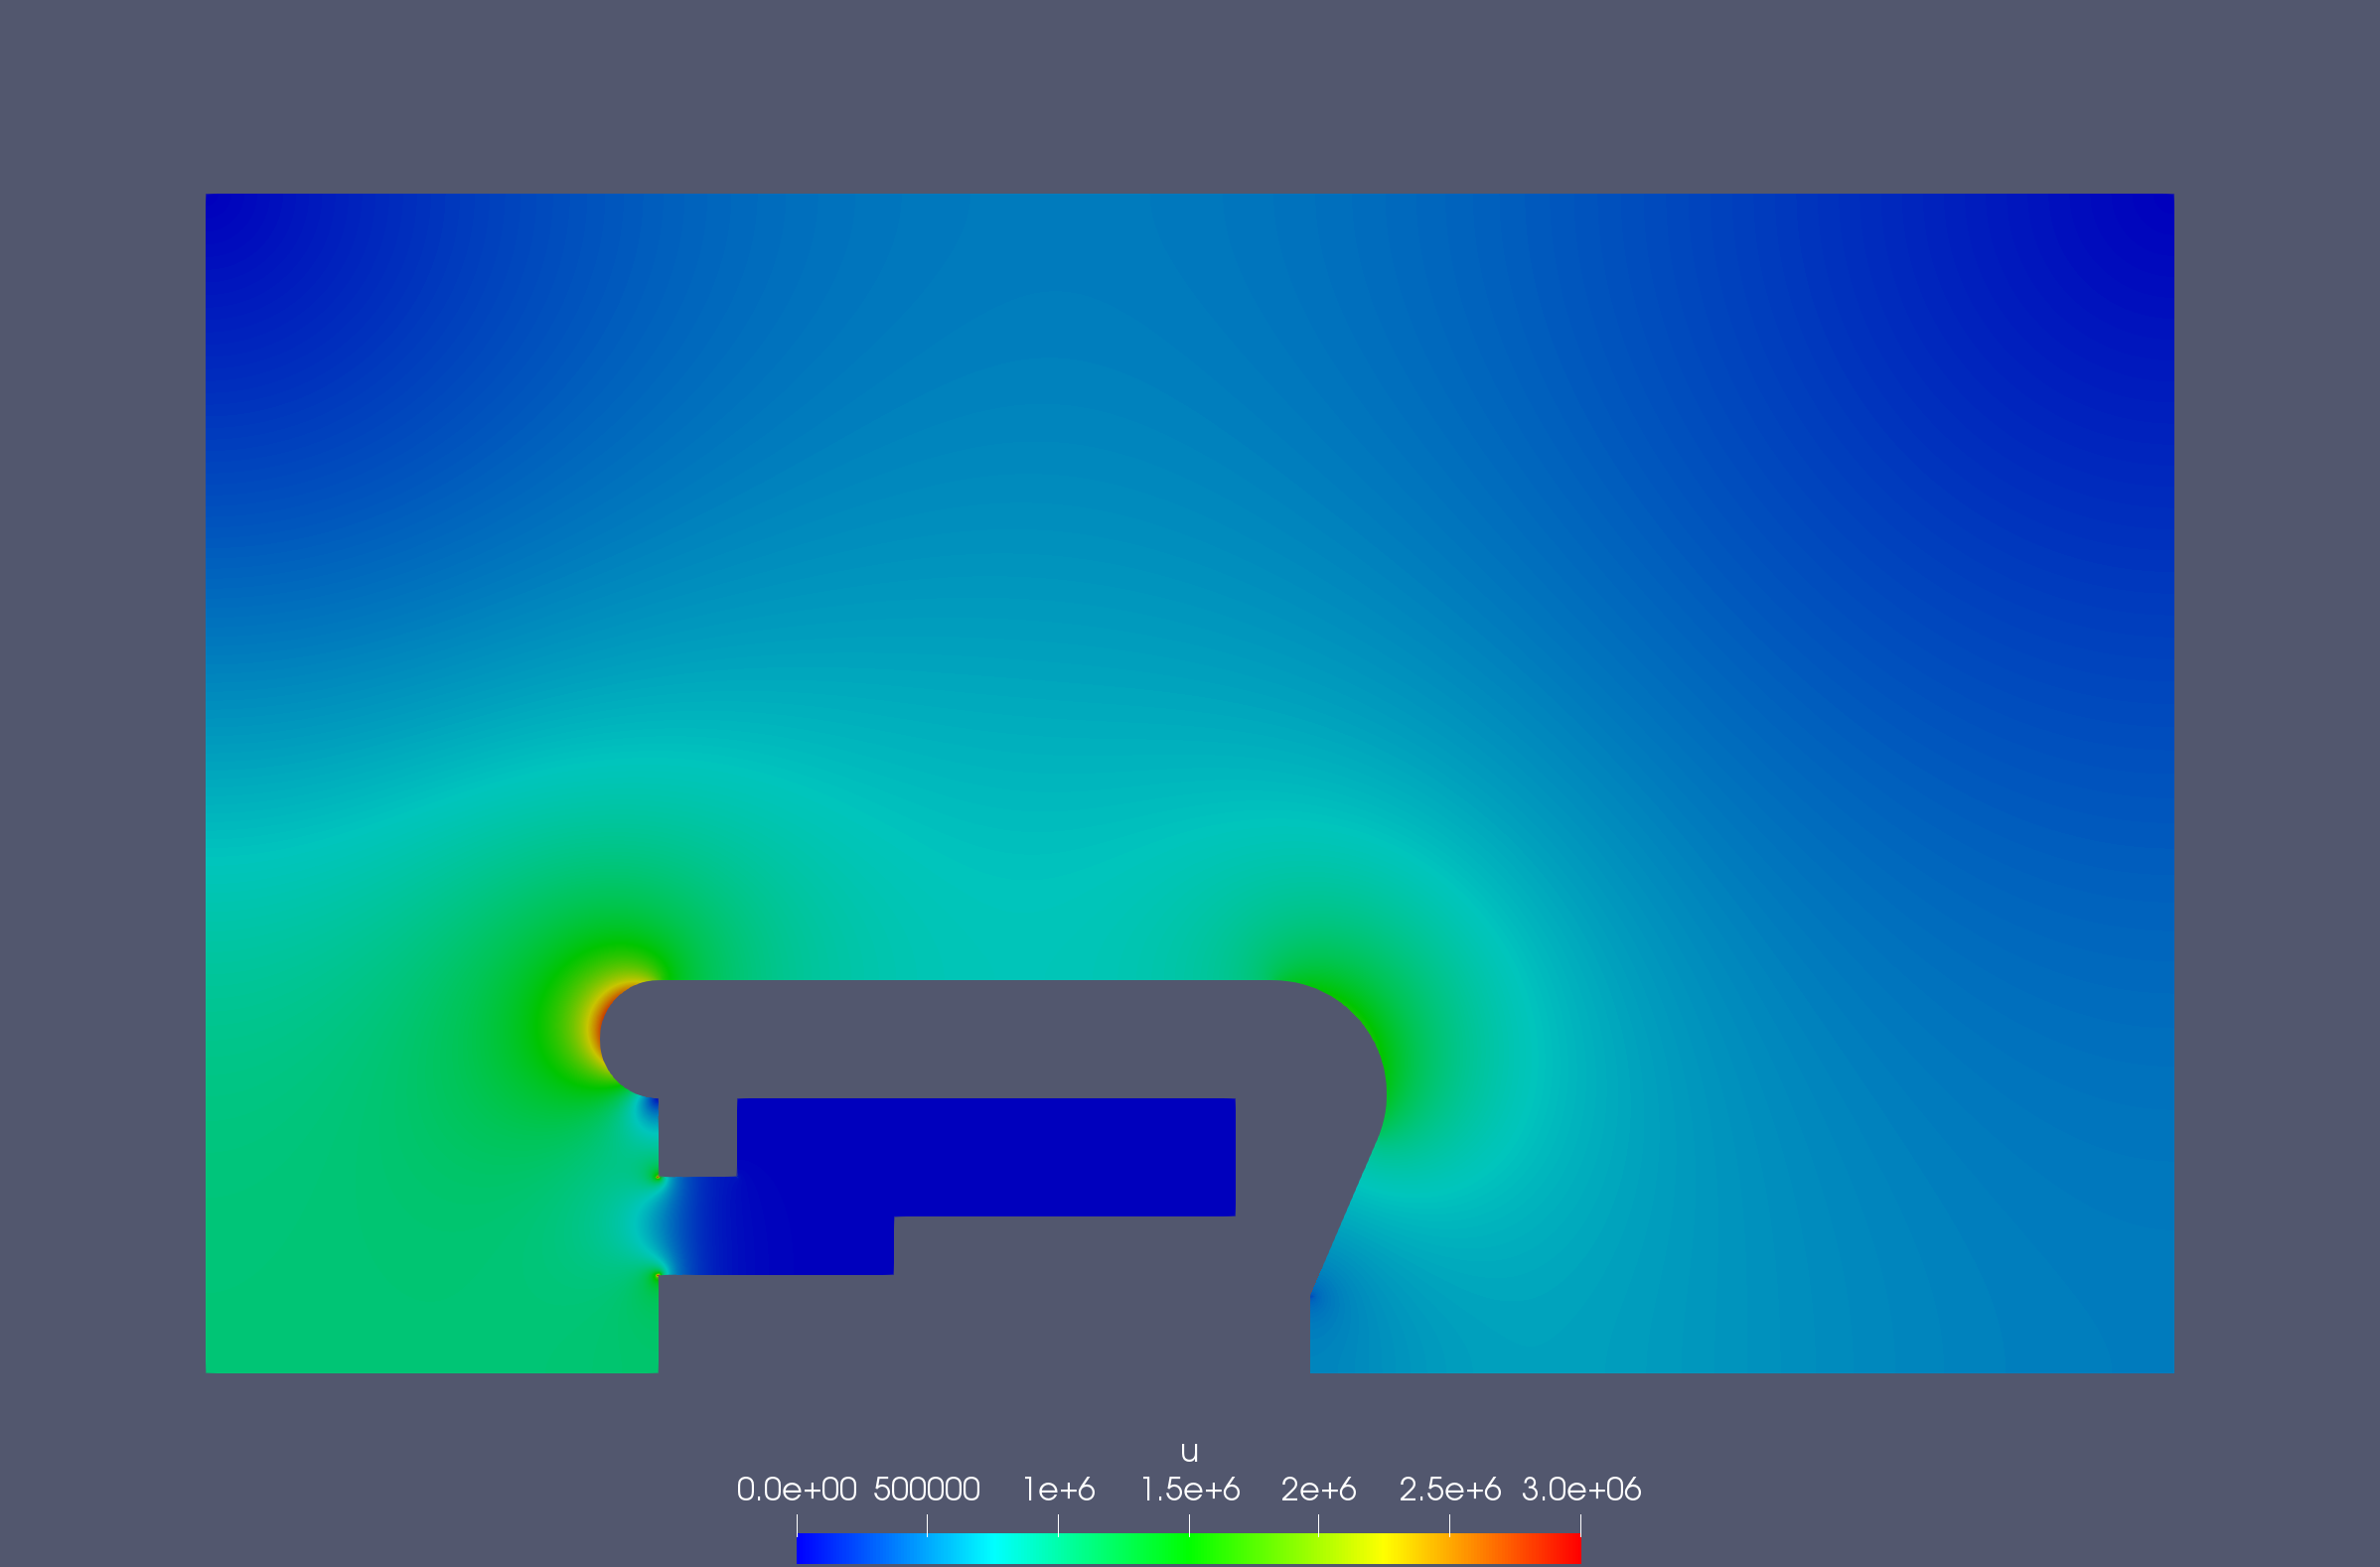
\includegraphics[width=\textwidth]{figures/60kV/gradient}
  \caption{Absolute value of the electric field.}
  \label{fig:electric_field}
\end{figure}
\end{center}

\begin{center}
\begin{figure}[H]
  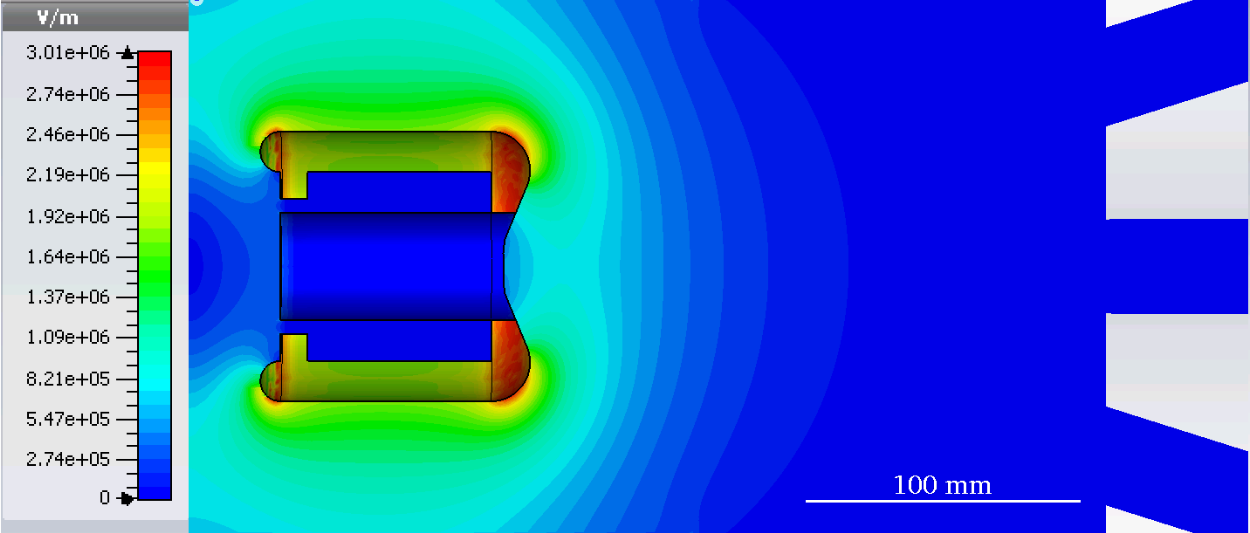
\includegraphics[width=\textwidth]{figures/60kV/electric_field}
  \caption{Results from the PhD thesis.}
  \label{fig:phd_electric_field}
\end{figure}
\end{center}

\begin{center}
\begin{figure}[H]
  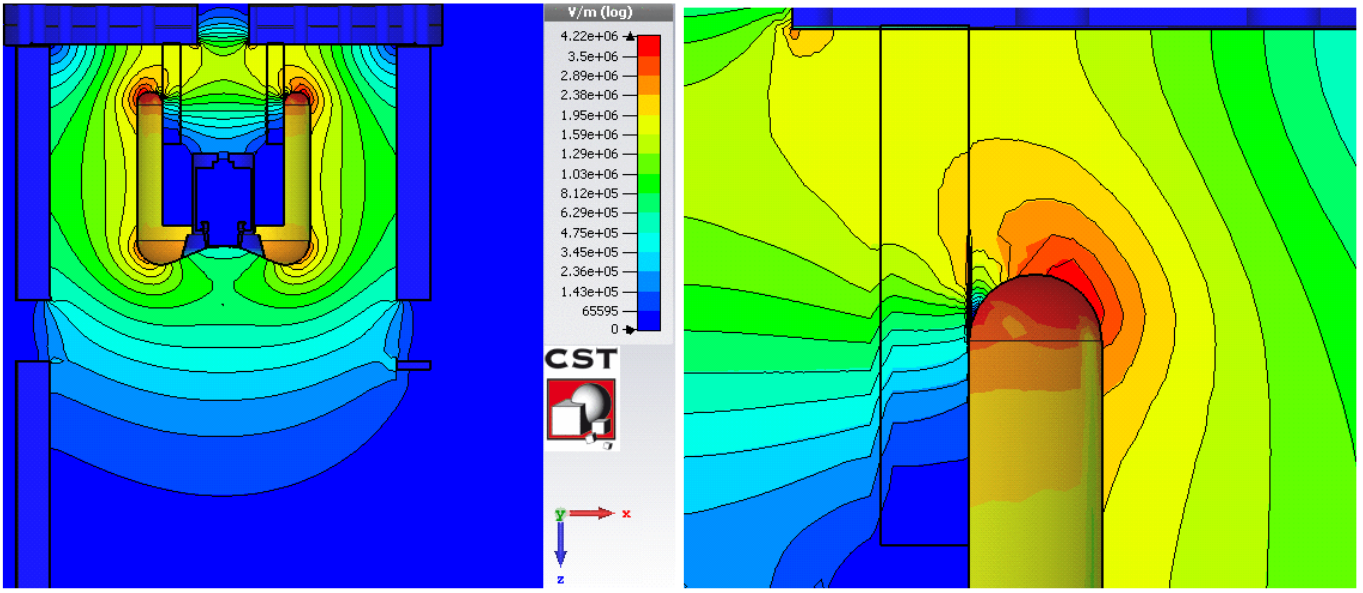
\includegraphics[width=\textwidth]{figures/60kV/electric_field_wende}
  \caption{Results from the Bachelor thesis.}
  \label{fig:electric_field_wende}
\end{figure}
\end{center}

\subsection{Convergence Study}
The convergence studies investigate the accuracy of the solution while increasing the number of elements per patch. (Akin to $h$-refinement in classical FEA) Since no analytic solution exists we used a reference with $n_\mathrm{sub}=256$ and $p=4$ as a comparison.
The errors are computed as
\begin{align}
  e_{L^2} = \frac{\| \varphi_\mathrm{it} - \varphi_\mathrm{ref} \|_{L^2}}{\| \varphi_\mathrm{ref} \|_{L^2}}\\
  e_{H^1} = \frac{\| \varphi_\mathrm{it} - \varphi_\mathrm{ref} \|_{H^1}}{\| \varphi_\mathrm{ref} \|_{H^1}}
\end{align}
where
\begin{align}
  \| \varphi \|_{H^1} = \sqrt{ \| \varphi \|_{L^2}^2 + \| \nabla\varphi \|_{L^2}^2 }.
\end{align}
Here $\varphi$ denotes the electrostatic potential. The integrals associated with the $L^2$-norm are evaluated using a quadrature rule defined on each element of a given patch.

The degrees of the basis functions are given in the legend, as well as theoretical limits for the convergence rates. They are given by $p+1$ in the case of the $L^2$-norm (electrostatic potential) and $p$ in the case of the $H^1$-norm (electric field). As seen in fig.~\ref{fig:convergence_potential} and fig.~\ref{fig:convergence_gradient} we observe convergence, however the convergence rate appears to be limited.

\begin{figure}[H]
  \begin{center}
    \begin{tikzpicture}

\begin{loglogaxis}[
   scale only axis = true,
   width = 0.7\textwidth,
   try min ticks=4,
   max space between ticks=1000pt,
  xlabel={$1/n_\mathrm{sub}$},
  ylabel={$e_{L^2}$},
  legend entries={$p=1$, $h^{1+1}$, $p=2$, $h^{2+1}$, $p=3$, $h^{3+1}$},
  legend pos=outer north east]

\addplot [color=brewerred] table[x=h, y=errl2]{figures/60kV/convergence/photocathode_insulator_degree_ref=4_nsub_ref=128_nquad_offset_ref=4_degree=1_N_it=7_nquad=0.dat};

\addplot [color=brewergrey] table[x=h, y=h_l2]{figures/60kV/convergence/photocathode_insulator_degree_ref=4_nsub_ref=128_nquad_offset_ref=4_degree=1_N_it=7_nquad=0.dat};

\addplot [color=brewerblue] table[x=h, y=errl2]{figures/60kV/convergence/photocathode_insulator_degree_ref=4_nsub_ref=128_nquad_offset_ref=4_degree=2_N_it=7_nquad=0.dat};

\addplot [color=brewergrey] table[x=h, y=h_l2]{figures/60kV/convergence/photocathode_insulator_degree_ref=4_nsub_ref=128_nquad_offset_ref=4_degree=2_N_it=7_nquad=0.dat};

\addplot [color=brewergreen] table[x=h, y=errl2]{figures/60kV/convergence/photocathode_insulator_degree_ref=4_nsub_ref=256_nquad_offset_ref=4_degree=3_N_it=8_nquad=0.dat};

\addplot [color=brewergrey] table[x=h, y=h_l2]{figures/60kV/convergence/photocathode_insulator_degree_ref=4_nsub_ref=256_nquad_offset_ref=4_degree=3_N_it=8_nquad=0.dat};
\end{loglogaxis}
\end{tikzpicture}

    \caption{Convergence of $L^2$-norm.}
    \label{fig:convergence_potential}
  \end{center}
\end{figure}

\begin{figure}[H]
  \begin{center}
    \begin{tikzpicture}

\begin{loglogaxis}[
  xlabel={$1/n_\mathrm{sub}$},
  ylabel={$e_{H^1}$},
  legend entries={$p=2$, $h^{2}$, $p=3$, $h^{3}$, $p=4$, $h^{4}$},
  legend pos=outer north east]

\addplot [color=brewerred] table[x=h, y=errh1]{figures/insulator/convergence/convergence_ref=5_degree=2.dat};

\addplot [color=brewergrey] table[x=h, y=h_h1]{figures/insulator/convergence/convergence_ref=5_degree=2.dat};

\addplot [color=brewerblue] table[x=h, y=errh1]{figures/insulator/convergence/convergence_ref=5_degree=3.dat};

\addplot [color=brewergrey] table[x=h, y=h_h1]{figures/insulator/convergence/convergence_ref=5_degree=3.dat};

\addplot [color=brewergreen] table[x=h, y=errh1]{figures/insulator/convergence/convergence_ref=5_degree=4.dat};

\addplot [color=brewergrey] table[x=h, y=h_h1]{figures/insulator/convergence/convergence_ref=5_degree=4.dat};

\end{loglogaxis}
\end{tikzpicture}

    \caption{Convergence of $H^1$-norm.}
    \label{fig:convergence_gradient}
  \end{center}
\end{figure}

Lastly the error in specific regions of the geometry was investigated by displaying the absolute error of the eletric field on every individual element of the mesh. In the case of fig.~\ref{fig:error_elem} we chose $n_\mathrm{sub}=256$ and $p=3$ for the iterative solution and computed the errors with respect to a reference using $n_\mathrm{sub}=256$ and $p=4$.
The figure shows the absolute error on each element in a logarithmic scale. We observe that the errors are largest near sharp corners or large changes in the sizes of the mesh's elements. This is to be expected and as indicated by the colorbar the largest absolute errors come out to be around $19\ \mathrm{V/m}$ with the associated field magnitudes being almost exclusively larger than $10\ \mathrm{MV/m}$.

\begin{center}
\begin{figure}[H]
  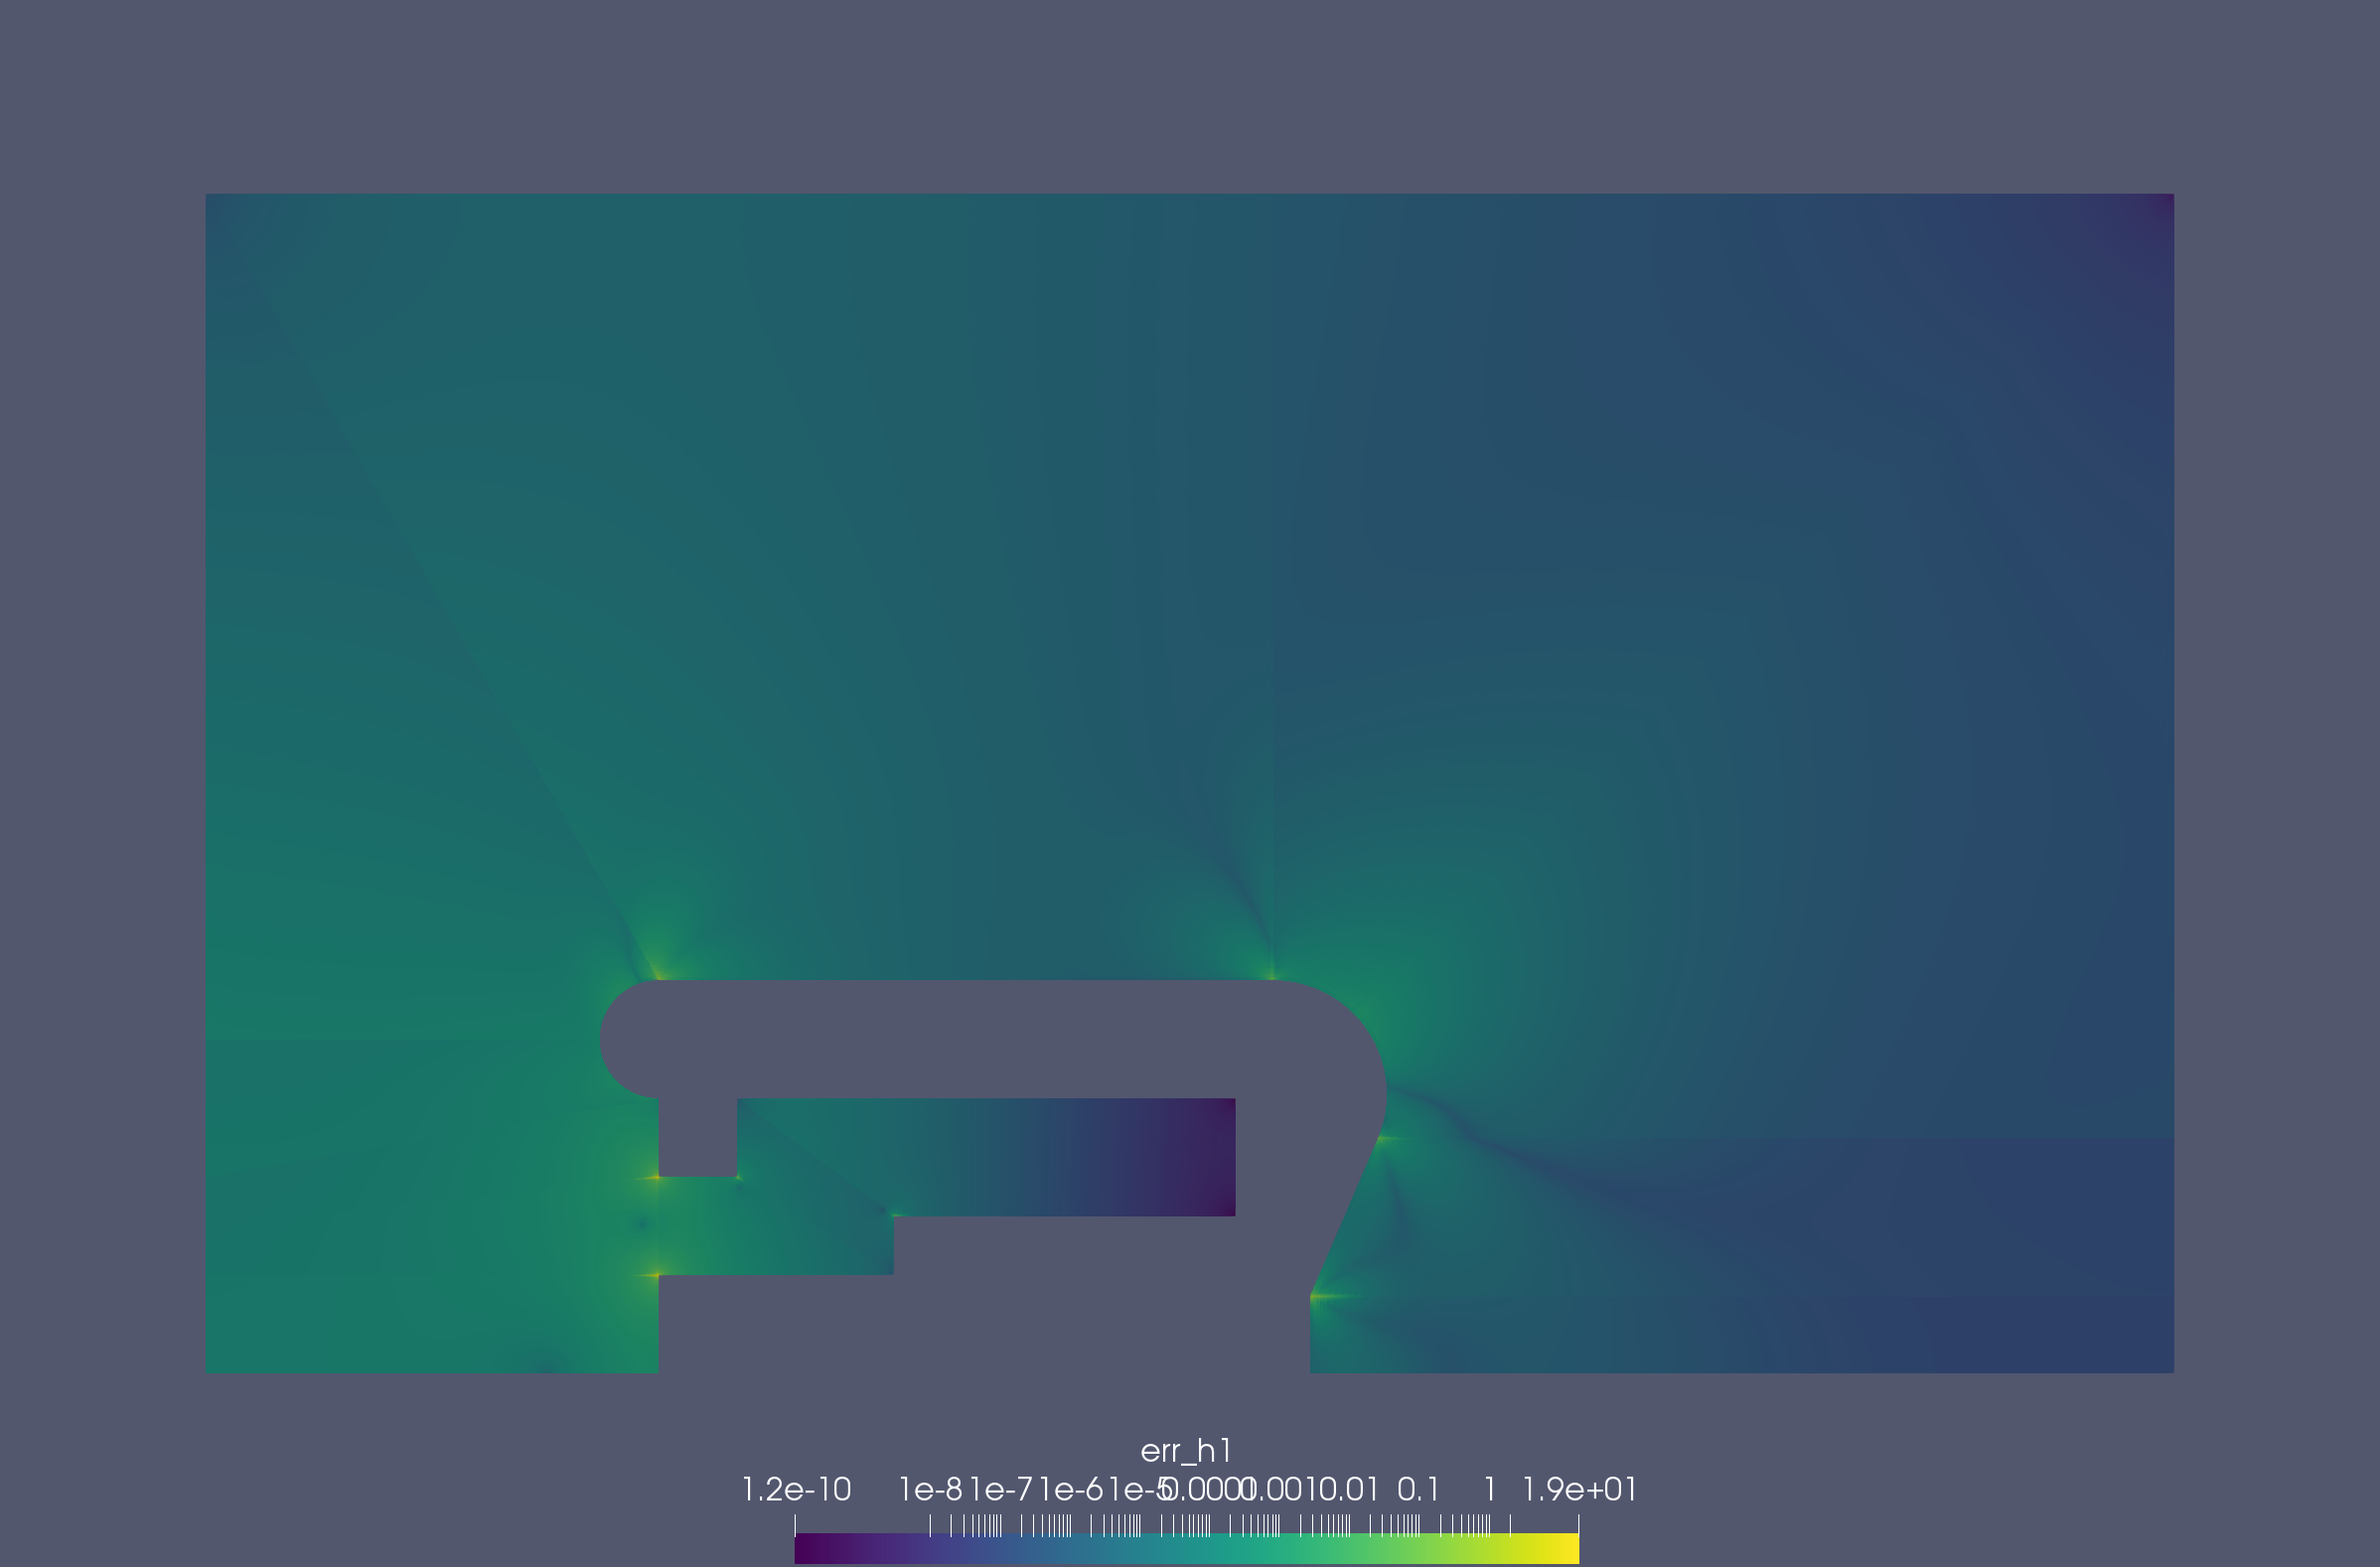
\includegraphics[width=\textwidth]{figures/60kV/error_elem}
  \caption{Absolute error of the electric field on every element.}
  \label{fig:error_elem}
\end{figure}
\end{center}


\section{200 kV Geometry}
\subsection{Geometry}
The $200$ kV geometry was derived from version one of the CST model. Some simplifications were made such that the geometry may be considered rotationally symmetric. The dimensions of the electrode, puck, puck elevator, vacuum chamber and insulator were derived from the model as depicted in fig.~\ref{fig:cst_geometry_yz}. The boundary conditions remained the same, except for the increase in voltage, when compared to the $60$ kV variant and the relative permittivity of the insulator was taken from the model to be $9.4$.

The geometry is depicted in fig.~\ref{fig:200kV_geometry_v1}. The numbers refer to the individual patches in the context of IGA. The patch boundaries are indicated by grey lines. The red lines represent homogeneous Dirichlet boundary conditions, the blue lines inhomogeneous Dirichlet boundary conditions with a value of $-200$ kV and the black lines indicate homogeneous Neumann boundaries.
The patches containing insulator material are colored in red.

\begin{center}
\begin{figure}[H]
   \begin{subfigure}{0.45\textwidth}
      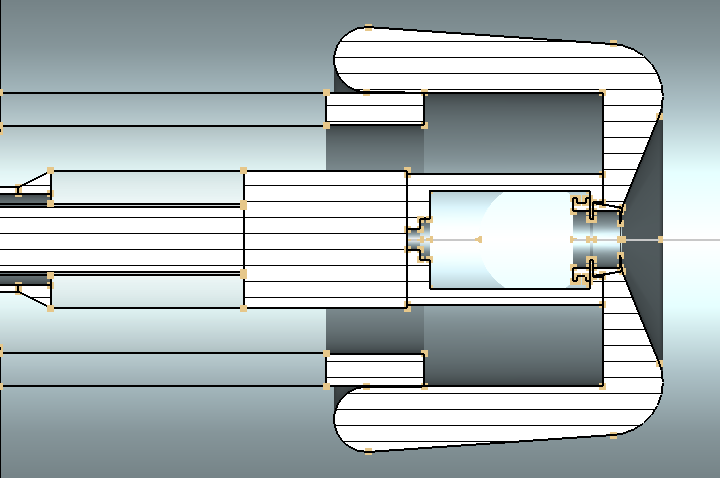
\includegraphics[width=\textwidth]{figures/200kV/png/v1_cutx}
      \caption{$y$-$z$ view of the CST model for $x=0$.}
      \label{fig:cst_geometry_yz}
   \end{subfigure}
   \begin{subfigure}{0.45\textwidth}
      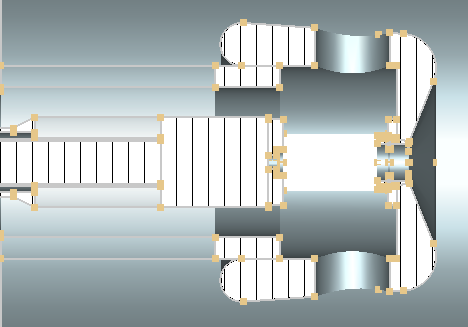
\includegraphics[width=\textwidth]{figures/200kV/png/v1_cuty}
      \caption{$x$-$z$ view of the CST model for $y=0$.}
      \label{fig:cst_geometry_xz}
   \end{subfigure}
\end{figure}
\end{center}

\begin{center}
\begin{figure}[H]
  \begin{tikzpicture}
\begin{axis}[
   scale only axis = true,
   width = 0.9\textwidth,
  axis equal,
  try min ticks=4,
  max space between ticks=1000pt,
  enlargelimits=true,
  colormap/Greens,
  point meta min = 0,
  point meta max = 2,
  x unit=m,
  y unit=m]

  \addplot[surf, shader=interp] table[point meta=\thisrow{c}]{figures/200kV/geometry/v1/geometry1.dat};

  \addplot[surf, shader=interp] table[point meta=\thisrow{c}]{figures/200kV/geometry/v1/geometry2.dat};

  \addplot[surf, shader=interp] table[point meta=\thisrow{c}]{figures/200kV/geometry/v1/geometry3.dat};

  \addplot[surf, shader=interp] table[point meta=\thisrow{c}]{figures/200kV/geometry/v1/geometry4.dat};

  \addplot[surf, shader=interp] table[point meta=\thisrow{c}]{figures/200kV/geometry/v1/geometry5.dat};

  \addplot[surf, shader=interp] table[point meta=\thisrow{c}]{figures/200kV/geometry/v1/geometry6.dat};

  \addplot[surf, shader=interp] table[point meta=\thisrow{c}]{figures/200kV/geometry/v1/geometry7.dat};

  \addplot[surf, shader=interp, colormap/Blues, point meta min = 0, point meta max = 1] table[point meta=\thisrow{c}]{figures/200kV/geometry/v1/geometry8.dat};

  \addplot[surf, shader=interp] table[point meta=\thisrow{c}]{figures/200kV/geometry/v1/geometry9.dat};

  \addplot[surf, shader=interp] table[point meta=\thisrow{c}]{figures/200kV/geometry/v1/geometry10.dat};

  \addplot[surf, shader=interp] table[point meta=\thisrow{c}]{figures/200kV/geometry/v1/geometry11.dat};

  \addplot[surf, shader=interp] table[point meta=\thisrow{c}]{figures/200kV/geometry/v1/geometry12.dat};

  \addplot[surf, shader=interp] table[point meta=\thisrow{c}]{figures/200kV/geometry/v1/geometry13.dat};

  \addplot[surf, shader=interp] table[point meta=\thisrow{c}]{figures/200kV/geometry/v1/geometry13.dat};

  \addplot[surf, shader=interp, colormap/Reds, point meta min = 0, point meta max = 1] table[point meta=\thisrow{c}]{figures/200kV/geometry/v1/geometry14.dat};

  \addplot[surf, shader=interp] table[point meta=\thisrow{c}]{figures/200kV/geometry/v1/geometry15.dat};

  \addplot[surf, shader=interp] table[point meta=\thisrow{c}]{figures/200kV/geometry/v1/geometry16.dat};

  \addplot[surf, shader=interp] table[point meta=\thisrow{c}]{figures/200kV/geometry/v1/geometry17.dat};

  \addplot[surf, shader=interp, colormap/Reds, point meta min = 0, point meta max = 1] table[point meta=\thisrow{c}]{figures/200kV/geometry/v1/geometry18.dat};

  \addplot[surf, shader=interp, colormap/Reds, point meta min = 0, point meta max = 1] table[point meta=\thisrow{c}]{figures/200kV/geometry/v1/geometry19.dat};

  \addplot[surf, shader=interp] table[point meta=\thisrow{c}]{figures/200kV/geometry/v1/geometry20.dat};

  \addplot[surf, shader=interp] table[point meta=\thisrow{c}]{figures/200kV/geometry/v1/geometry21.dat};

  \addplot[surf, shader=interp] table[point meta=\thisrow{c}]{figures/200kV/geometry/v1/geometry22.dat};

  \addplot[surf, shader=interp] table[point meta=\thisrow{c}]{figures/200kV/geometry/v1/geometry23.dat};

  \addplot[surf, shader=interp] table[point meta=\thisrow{c}]{figures/200kV/geometry/v1/geometry24.dat};

  % add patch indices
  \addplot[only marks, point meta=explicit symbolic, color=black, nodes near coords] coordinates{
  (0.28,-0.01) [(1)]
  (0.28,-0.005) [(2)]
  (0.28,0.005) [(3)]
  (0.28,0.015) [(4)]
  (0.28,0.045) [(5)]
  (0.24,0.075) [(6)]
  (0.185,0.075) [(7)]
  (0.165,0.075) [(8)]
  (0.125,0.075) [(9)]
  (0.095,0.065) [(10)]
  (0.1,0.04) [(11)]
  (0.05,0.075) [(12)]
  (0.06,0.045) [(13)]
  (0.05,0.03) [(14)]
  (0.03,0.02) [(15)]
  (0.07,0.017) [(16)]
  (0.005,0.01) [(17)]
  (0.055,0.007) [(18)]
  (0.007,0.004) [(19)]
  (0.035,-0.005) [(20)]
  (0.11,0.017) [(21)]
  (0.17,0.01) [(22)]
  (0.135,0.0175) [(23)]
  (0.165,0.0275) [(24)]
  };

  % add patch boundaries
  \addplot[color=brewerblue] table{figures/200kV/boundary/v1/boundaries11.dat};
  \addplot[color=brewerred] table{figures/200kV/boundary/v1/boundaries12.dat};
  \addplot[color=black] table{figures/200kV/boundary/v1/boundaries13.dat};
  \addplot[color=brewergrey] table{figures/200kV/boundary/v1/boundaries14.dat};

  \addplot[color=brewerblue] table{figures/200kV/boundary/v1/boundaries21.dat};
  \addplot[color=brewerred] table{figures/200kV/boundary/v1/boundaries22.dat};
  \addplot[color=brewergrey] table{figures/200kV/boundary/v1/boundaries23.dat};
  \addplot[color=brewergrey] table{figures/200kV/boundary/v1/boundaries24.dat};

  \addplot[color=brewerblue] table{figures/200kV/boundary/v1/boundaries31.dat};
  \addplot[color=brewerred] table{figures/200kV/boundary/v1/boundaries32.dat};
  \addplot[color=brewergrey] table{figures/200kV/boundary/v1/boundaries33.dat};
  \addplot[color=brewergrey] table{figures/200kV/boundary/v1/boundaries34.dat};

  \addplot[color=brewerblue] table{figures/200kV/boundary/v1/boundaries41.dat};
  \addplot[color=brewerred] table{figures/200kV/boundary/v1/boundaries42.dat};
  \addplot[color=brewergrey] table{figures/200kV/boundary/v1/boundaries43.dat};
  \addplot[color=brewergrey] table{figures/200kV/boundary/v1/boundaries44.dat};

  \addplot[color=brewerblue] table{figures/200kV/boundary/v1/boundaries51.dat};
  \addplot[color=brewerred] table{figures/200kV/boundary/v1/boundaries52.dat};
  \addplot[color=brewergrey] table{figures/200kV/boundary/v1/boundaries53.dat};
  \addplot[color=brewergrey] table{figures/200kV/boundary/v1/boundaries54.dat};

  \addplot[color=brewergrey] table{figures/200kV/boundary/v1/boundaries61.dat};
  \addplot[color=brewergrey] table{figures/200kV/boundary/v1/boundaries62.dat};
  \addplot[color=brewerblue] table{figures/200kV/boundary/v1/boundaries63.dat};
  \addplot[color=brewerred] table{figures/200kV/boundary/v1/boundaries64.dat};

  \addplot[color=brewergrey] table{figures/200kV/boundary/v1/boundaries71.dat};
  \addplot[color=brewergrey] table{figures/200kV/boundary/v1/boundaries72.dat};
  \addplot[color=brewerblue] table{figures/200kV/boundary/v1/boundaries73.dat};
  \addplot[color=brewerred] table{figures/200kV/boundary/v1/boundaries74.dat};

  \addplot[color=brewergrey] table{figures/200kV/boundary/v1/boundaries81.dat};
  \addplot[color=brewergrey] table{figures/200kV/boundary/v1/boundaries82.dat};
  \addplot[color=brewerblue] table{figures/200kV/boundary/v1/boundaries83.dat};
  \addplot[color=brewerred] table{figures/200kV/boundary/v1/boundaries84.dat};

  \addplot[color=brewergrey] table{figures/200kV/boundary/v1/boundaries91.dat};
  \addplot[color=brewergrey] table{figures/200kV/boundary/v1/boundaries92.dat};
  \addplot[color=brewerblue] table{figures/200kV/boundary/v1/boundaries93.dat};
  \addplot[color=brewerred] table{figures/200kV/boundary/v1/boundaries94.dat};

  \addplot[color=brewergrey] table{figures/200kV/boundary/v1/boundaries101.dat};
  \addplot[color=brewerblue] table{figures/200kV/boundary/v1/boundaries102.dat};
  \addplot[color=brewergrey] table{figures/200kV/boundary/v1/boundaries103.dat};
  \addplot[color=brewergrey] table{figures/200kV/boundary/v1/boundaries104.dat};

  \addplot[color=brewergrey] table{figures/200kV/boundary/v1/boundaries111.dat};
  \addplot[color=brewerblue] table{figures/200kV/boundary/v1/boundaries112.dat};
  \addplot[color=brewerblue] table{figures/200kV/boundary/v1/boundaries113.dat};
  \addplot[color=brewergrey] table{figures/200kV/boundary/v1/boundaries114.dat};

  \addplot[color=brewerred] table{figures/200kV/boundary/v1/boundaries121.dat};
  \addplot[color=brewergrey] table{figures/200kV/boundary/v1/boundaries122.dat};
  \addplot[color=brewergrey] table{figures/200kV/boundary/v1/boundaries123.dat};
  \addplot[color=brewerred] table{figures/200kV/boundary/v1/boundaries124.dat};

  \addplot[color=brewerred] table{figures/200kV/boundary/v1/boundaries131.dat};
  \addplot[color=brewergrey] table{figures/200kV/boundary/v1/boundaries132.dat};
  \addplot[color=brewergrey] table{figures/200kV/boundary/v1/boundaries133.dat};
  \addplot[color=brewergrey] table{figures/200kV/boundary/v1/boundaries134.dat};

  \addplot[color=brewerred] table{figures/200kV/boundary/v1/boundaries141.dat};
  \addplot[color=brewerblue] table{figures/200kV/boundary/v1/boundaries142.dat};
  \addplot[color=brewergrey] table{figures/200kV/boundary/v1/boundaries143.dat};
  \addplot[color=brewergrey] table{figures/200kV/boundary/v1/boundaries144.dat};

  \addplot[color=brewerred] table{figures/200kV/boundary/v1/boundaries151.dat};
  \addplot[color=brewergrey] table{figures/200kV/boundary/v1/boundaries152.dat};
  \addplot[color=brewergrey] table{figures/200kV/boundary/v1/boundaries153.dat};
  \addplot[color=brewergrey] table{figures/200kV/boundary/v1/boundaries154.dat};

  \addplot[color=brewergrey] table{figures/200kV/boundary/v1/boundaries161.dat};
  \addplot[color=brewergrey] table{figures/200kV/boundary/v1/boundaries162.dat};
  \addplot[color=brewergrey] table{figures/200kV/boundary/v1/boundaries163.dat};
  \addplot[color=brewerblue] table{figures/200kV/boundary/v1/boundaries164.dat};

  \addplot[color=brewerred] table{figures/200kV/boundary/v1/boundaries171.dat};
  \addplot[color=brewergrey] table{figures/200kV/boundary/v1/boundaries172.dat};
  \addplot[color=brewergrey] table{figures/200kV/boundary/v1/boundaries173.dat};
  \addplot[color=brewergrey] table{figures/200kV/boundary/v1/boundaries174.dat};

  \addplot[color=brewergrey] table{figures/200kV/boundary/v1/boundaries181.dat};
  \addplot[color=brewerblue] table{figures/200kV/boundary/v1/boundaries182.dat};
  \addplot[color=brewergrey] table{figures/200kV/boundary/v1/boundaries183.dat};
  \addplot[color=brewergrey] table{figures/200kV/boundary/v1/boundaries184.dat};

  \addplot[color=brewerred] table{figures/200kV/boundary/v1/boundaries191.dat};
  \addplot[color=brewergrey] table{figures/200kV/boundary/v1/boundaries192.dat};
  \addplot[color=brewergrey] table{figures/200kV/boundary/v1/boundaries193.dat};
  \addplot[color=brewergrey] table{figures/200kV/boundary/v1/boundaries194.dat};

  \addplot[color=brewerred] table{figures/200kV/boundary/v1/boundaries201.dat};
  \addplot[color=brewerblue] table{figures/200kV/boundary/v1/boundaries202.dat};
  \addplot[color=black] table{figures/200kV/boundary/v1/boundaries203.dat};
  \addplot[color=brewergrey] table{figures/200kV/boundary/v1/boundaries204.dat};

  \addplot[color=brewergrey] table{figures/200kV/boundary/v1/boundaries211.dat};
  \addplot[color=brewergrey] table{figures/200kV/boundary/v1/boundaries212.dat};
  \addplot[color=brewerblue] table{figures/200kV/boundary/v1/boundaries213.dat};
  \addplot[color=brewerblue] table{figures/200kV/boundary/v1/boundaries214.dat};

  \addplot[color=brewerblue] table{figures/200kV/boundary/v1/boundaries221.dat};
  \addplot[color=brewerblue] table{figures/200kV/boundary/v1/boundaries222.dat};
  \addplot[color=brewerblue] table{figures/200kV/boundary/v1/boundaries223.dat};
  \addplot[color=brewergrey] table{figures/200kV/boundary/v1/boundaries224.dat};

  \addplot[color=brewergrey] table{figures/200kV/boundary/v1/boundaries231.dat};
  \addplot[color=brewerblue] table{figures/200kV/boundary/v1/boundaries232.dat};
  \addplot[color=brewergrey] table{figures/200kV/boundary/v1/boundaries233.dat};
  \addplot[color=brewergrey] table{figures/200kV/boundary/v1/boundaries234.dat};

  \addplot[color=brewerblue] table{figures/200kV/boundary/v1/boundaries241.dat};
  \addplot[color=brewerblue] table{figures/200kV/boundary/v1/boundaries242.dat};
  \addplot[color=brewergrey] table{figures/200kV/boundary/v1/boundaries243.dat};
  \addplot[color=brewerblue] table{figures/200kV/boundary/v1/boundaries244.dat};

\end{axis}
\end{tikzpicture}

  \caption{Refined 200 kV Photocathode geometry and boundary conditions.}
  \label{fig:200kV_geometry_v1}
\end{figure}
\end{center}

\subsection{Electric Field}
The solution for the electric field is shown in fig.~\ref{fig:200kV_electric_field}.
It was computed with $p=3$ as the degree of the basis functions and $n_\mathrm{sub}=16$ as the number of elements that each knot vector is uniformly split into. The fairly low number of subdomains was chosen to improve performance in regards to the optimization.
It is evident that there exist parts of the domain where the magnitude of the electric field is close to the limit of $10 \frac{\mathrm{MV}}{\mathrm{m}}$. There are also very high gradients visible at the triple points however these also coincide with sharp corners so numerical issues might play a role.

\begin{center}
\begin{figure}[H]
  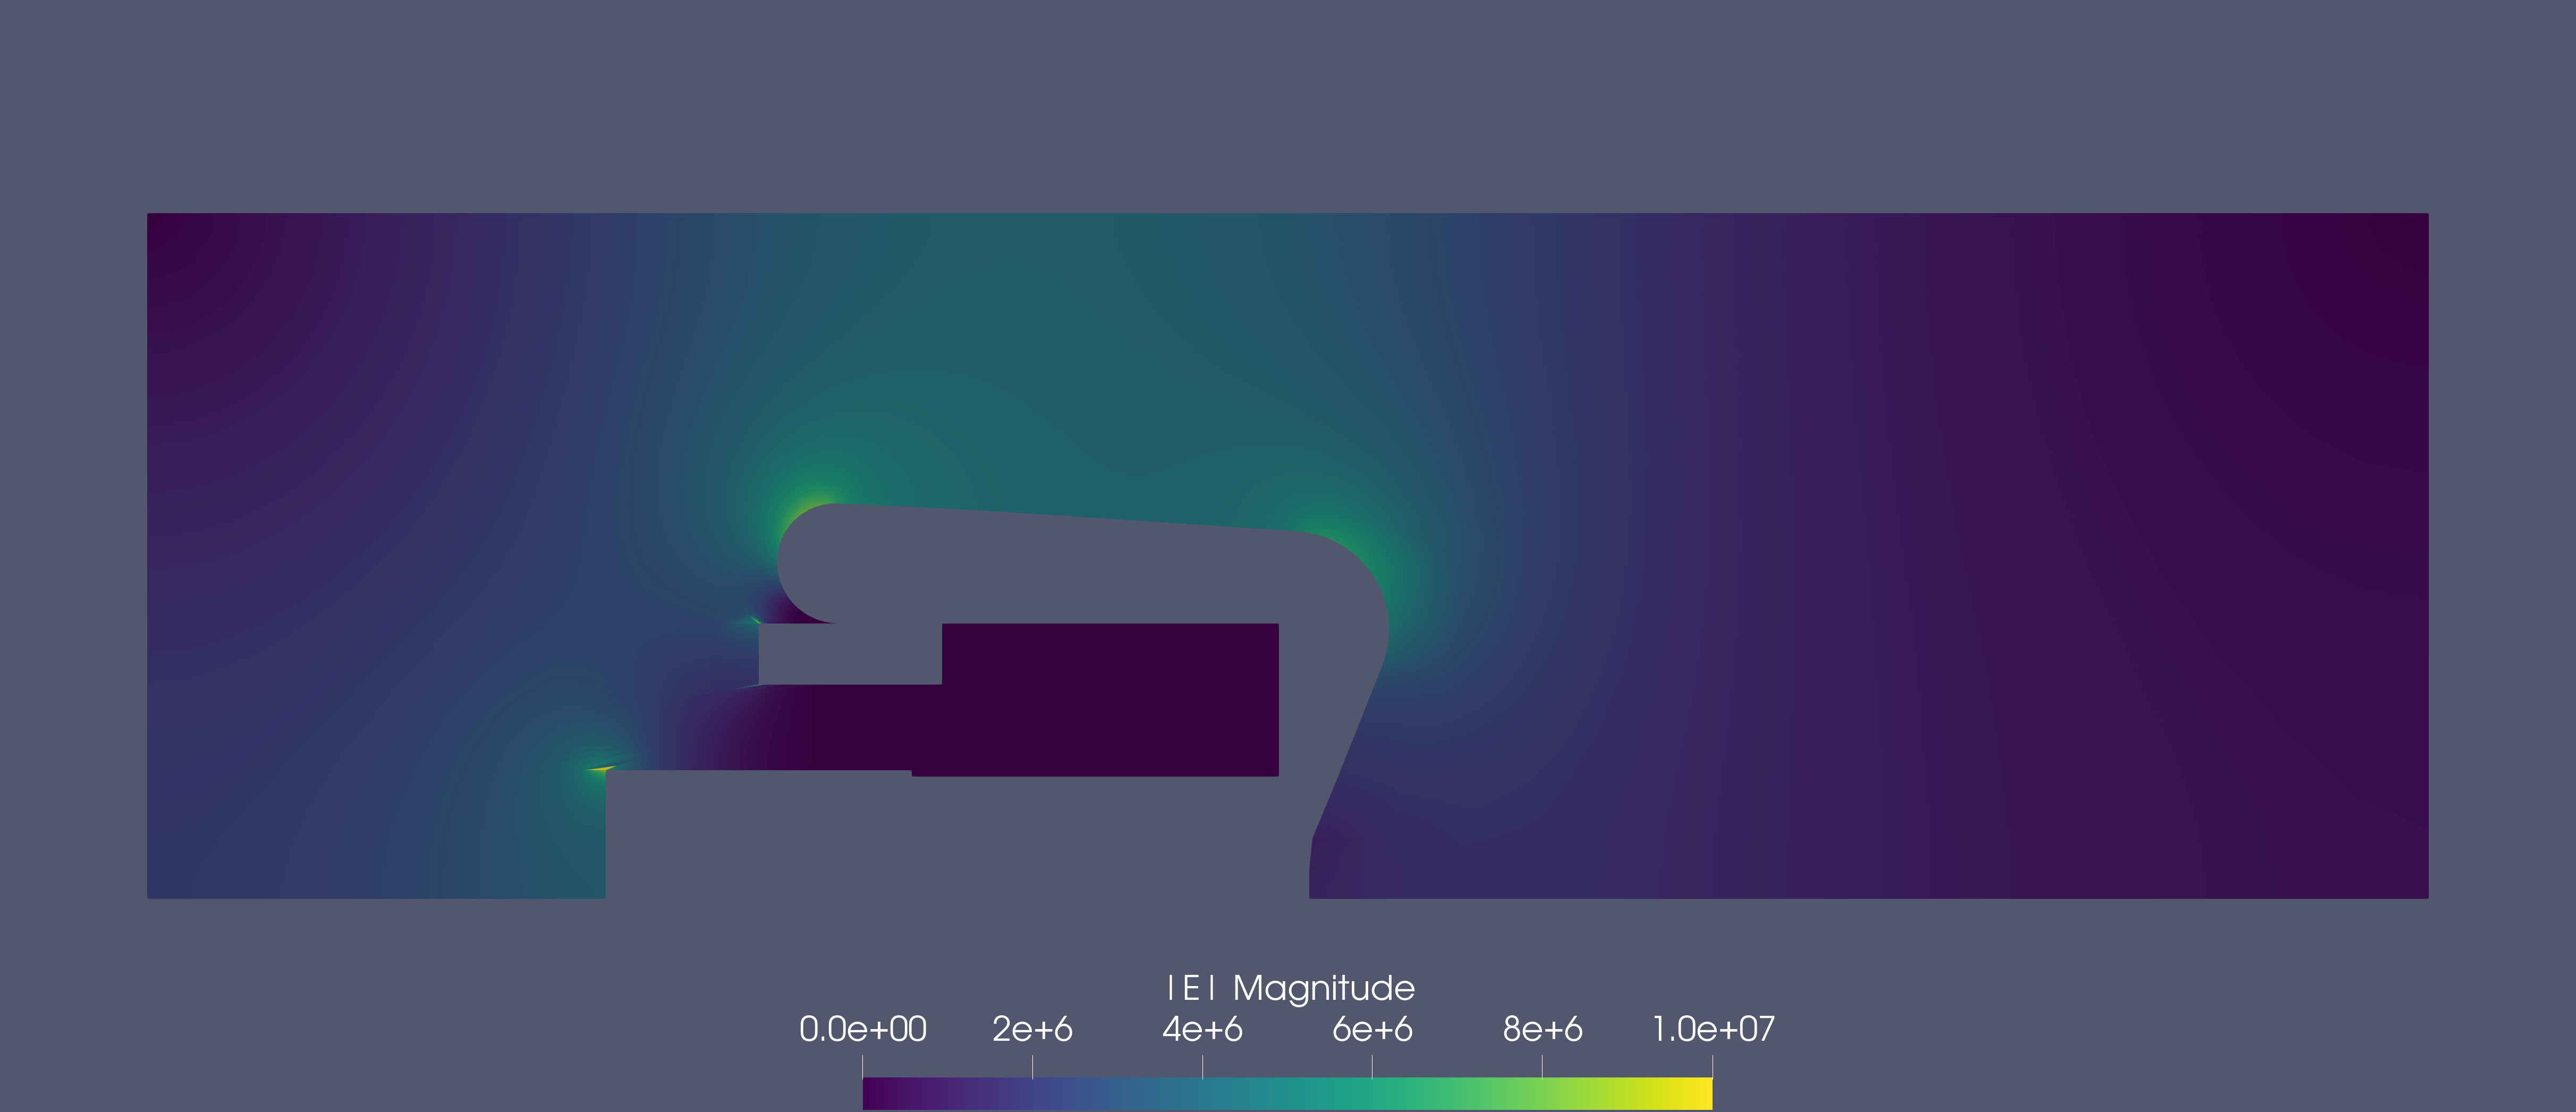
\includegraphics[width=\textwidth]{figures/200kV/png/order=3}
  \caption{Absolute value of the electric field with $p=3$ and $n_\mathrm{sub}=16$.}
  \label{fig:200kV_electric_field}
\end{figure}
\end{center}

\subsection{Optimization}
The aim of the optimization is to minimize the maximal field amplitudes. For practicality we will only look at the critical points of the geometry, i.~e.~the curvatures of the outer electrode and the triple points. The lower part of the geometry will remain fixed so only the electrode boundaries of patches 5 through 11 from fig.~\ref{fig:200kV_geometry_v1} and their respective control points are the DoFs. Aside from the fixed part of the geometry we also consider a volume constraint.

\subsubsection{Volume Constraint}
One of the constraints for the optimization is the weight of the electrode and thus its volume.
We first compute the volume of the patches by taking into account the rotational symmetry and discretizing $V_{\mathrm{ptc}} = \int_V r\ \drm r\ \drm \varphi\ \drm z$ via numerical quadrature. We can then obtain the volume of the electrode by subtracting $V_{\mathrm{ptc}}$ from the cylinder formed by the vacuumchamber.
We still need to consider the holes inside the electrode, visible in \ref{fig:cst_geometry_xz}. Their volume is computed by considering a cylinder with its height as a function of $z$. The curvature in $x$ and $y$ is disregarded, since it is the same for both coordinates. We can therefore determine the value by discretizing $V_{h} = \int_V \drm x\ \drm y\ \drm z$.
Lastly the connection of the electrode with the insulator as well as the lift and the connection to the cable are not part of the electrode and thus their volume is subtracted as well.
In total the physical constraint is set at $625\ \mathrm{cm}^3$ and the volume of the current geometry is computed as approximately $608\ \mathrm{cm}^3$.

\subsubsection{Cost Function}
For the cost function we first define $E_i$ as the maximal absolute electric field across the quadrature nodes of patch $i$.
We then define the cost function to be
\begin{align}
   C = \frac{1}{|I|} \sum_{i \in I} E_i
\end{align}
where $I$ contains the indices of the patches of interest.

\subsubsection{Additional Constraints}
As an additional constraint we require $C^1$ continuity of the section that is optimized. The starting nurbs is depicted in fig.~\ref{fig:nurbs}. Furthermore the control points, which represent the DOFs, are constrained to stay inside their respective patch boundaries. To correctly model the holes with patch 8 the adjacent control points are constrained to only move vertically.

\begin{center}
\begin{figure}[H]
  \begin{tikzpicture}
\begin{axis}[
   scale only axis = true,
   width = 0.45\textwidth,
   axis equal,
   try min ticks=4,
   max space between ticks=1000pt,
   enlargelimits=true,
   x unit=m,
   y unit=m]

   \addplot[color=brewergrey] table {figures/200kV/nurbs/nurbs_5_1.dat};
   \addplot[color=brewerred, mark=*] table {figures/200kV/nurbs/nurbs_5_1_coefs.dat};
   \addplot[color=brewergrey, dashed] table {figures/200kV/nurbs/nurbs_5_1_net.dat};

   \addplot[color=brewergrey] table {figures/200kV/nurbs/nurbs_6_3.dat};
   \addplot[color=brewerred, mark=*] table {figures/200kV/nurbs/nurbs_6_3_coefs.dat};
   \addplot[color=brewergrey, dashed] table {figures/200kV/nurbs/nurbs_6_3_net.dat};

   \addplot[color=brewergrey] table {figures/200kV/nurbs/nurbs_7_3.dat};
   \addplot[color=brewerred, mark=*] table {figures/200kV/nurbs/nurbs_7_3_coefs.dat};
   \addplot[color=brewergrey, dashed] table {figures/200kV/nurbs/nurbs_7_3_net.dat};

   \addplot[color=brewergrey] table {figures/200kV/nurbs/nurbs_8_3.dat};
   \addplot[color=brewerred, mark=*] table {figures/200kV/nurbs/nurbs_8_3_coefs.dat};
   \addplot[color=brewergrey, dashed] table {figures/200kV/nurbs/nurbs_8_3_net.dat};

   \addplot[color=brewergrey] table {figures/200kV/nurbs/nurbs_9_3.dat};
   \addplot[color=brewerred, mark=*] table {figures/200kV/nurbs/nurbs_9_3_coefs.dat};
   \addplot[color=brewergrey, dashed] table {figures/200kV/nurbs/nurbs_9_3_net.dat};

   \addplot[color=brewergrey] table {figures/200kV/nurbs/nurbs_10_2.dat};
   \addplot[color=brewerred, mark=*] table {figures/200kV/nurbs/nurbs_10_2_coefs.dat};
   \addplot[color=brewergrey, dashed] table {figures/200kV/nurbs/nurbs_10_2_net.dat};

   \addplot[color=brewergrey] table {figures/200kV/nurbs/nurbs_11_2.dat};
   \addplot[color=brewerred, mark=*] table {figures/200kV/nurbs/nurbs_11_2_coefs.dat};
   \addplot[color=brewergrey, dashed] table {figures/200kV/nurbs/nurbs_11_2_net.dat};
\end{axis}
\end{tikzpicture}

  \caption{$C^1$ continuous nurbs that is to be optimized including control points.}
  \label{fig:nurbs}
\end{figure}
\end{center}

\subsubsection{NLopt}
For the optimization we used implementations of BOBYQA and COBYLA as given by the NLopt libary. For now we selected to use COBYLA as it is able to directly handle nonlinear constraints whereas they need to be enforced using an augmented Lagrangian method for BOBYQA.

\subsubsection{Results}
The results obtained from the optimization are depicted in fig:~\ref{fig:results_iga}. For the cost function we chose $I=\{ 6, \dotsc, 11 \}$. The new geometry has a volume of about 625 $\mathrm{cm}^3$. The original value of the cost function was 6.2 $\frac{\mathrm{MV}}{\mathrm{m}}$ and the optimized one is 5.3 $\frac{\mathrm{MV}}{\mathrm{m}}$. The absolute maximum value in any of the quadrature points was 7.7 $\frac{\mathrm{MV}}{\mathrm{m}}$ to begin with and ended up at 6.1 $\frac{\mathrm{MV}}{\mathrm{m}}$.

\begin{center}
\begin{figure}[H]
  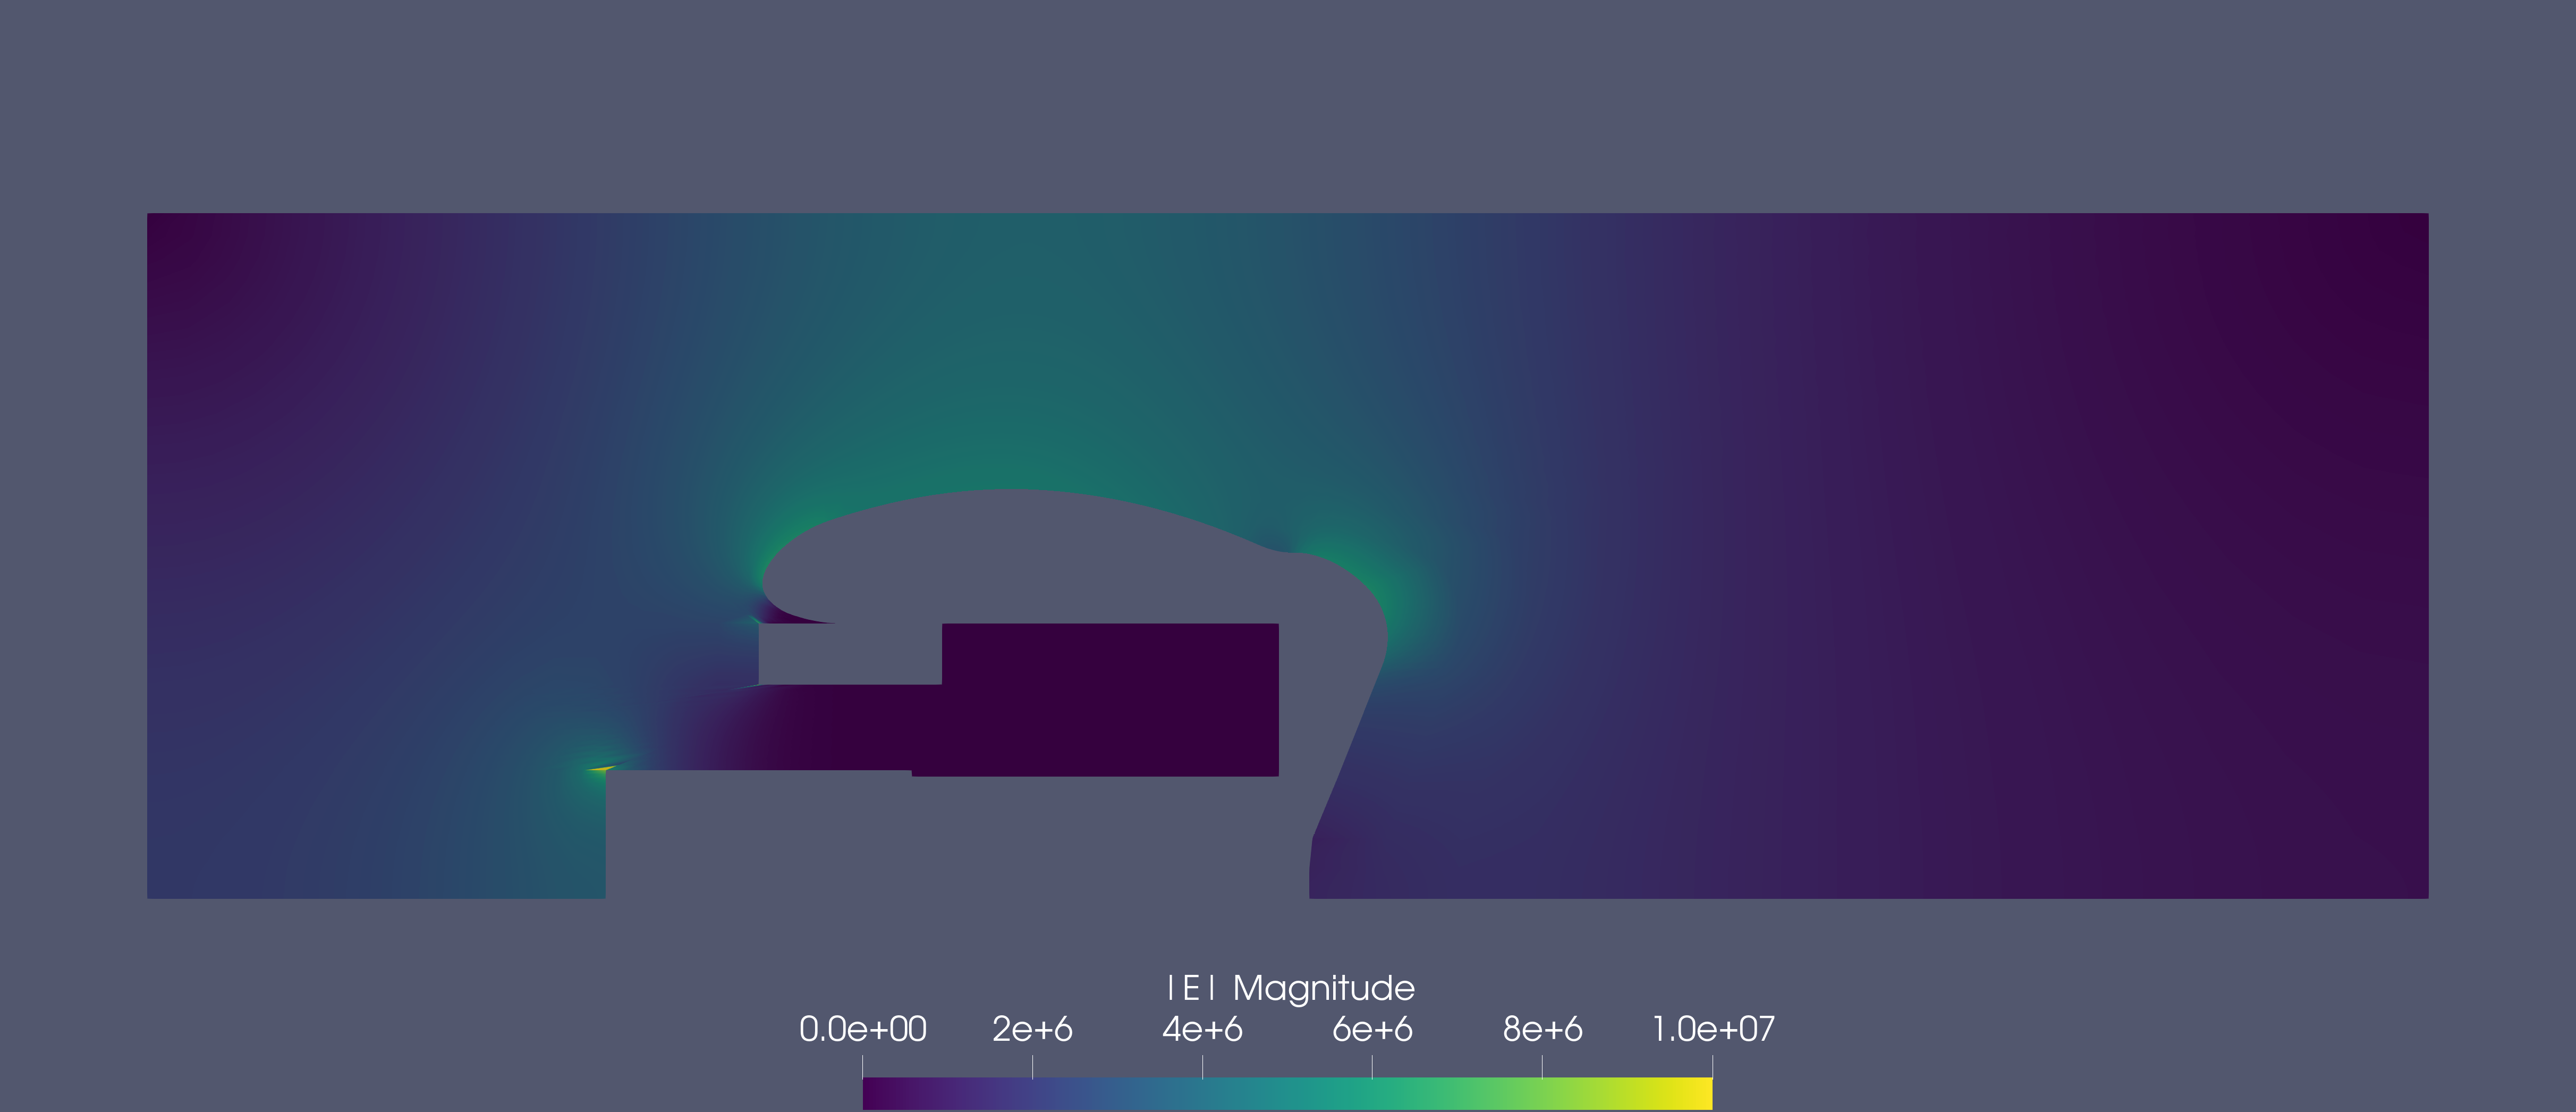
\includegraphics[width=\textwidth]{figures/200kV/png/cobyla_run11}
  \caption{Optimization result using COBYLA with $I=\{ 6, \dots, 11 \}$.}
  \label{fig:results_iga}
\end{figure}
\end{center}

In order to compare the results with the original geometry and simulation the optimized geometry was also imported and simulated in CST. The results visibly indicate a clear improvement from the optimized geometry over the original one. This is in agreement with the numerical improvement observed in the context of IGA.

\begin{center}
\begin{figure}[H]
   \begin{subfigure}{0.45\textwidth}
      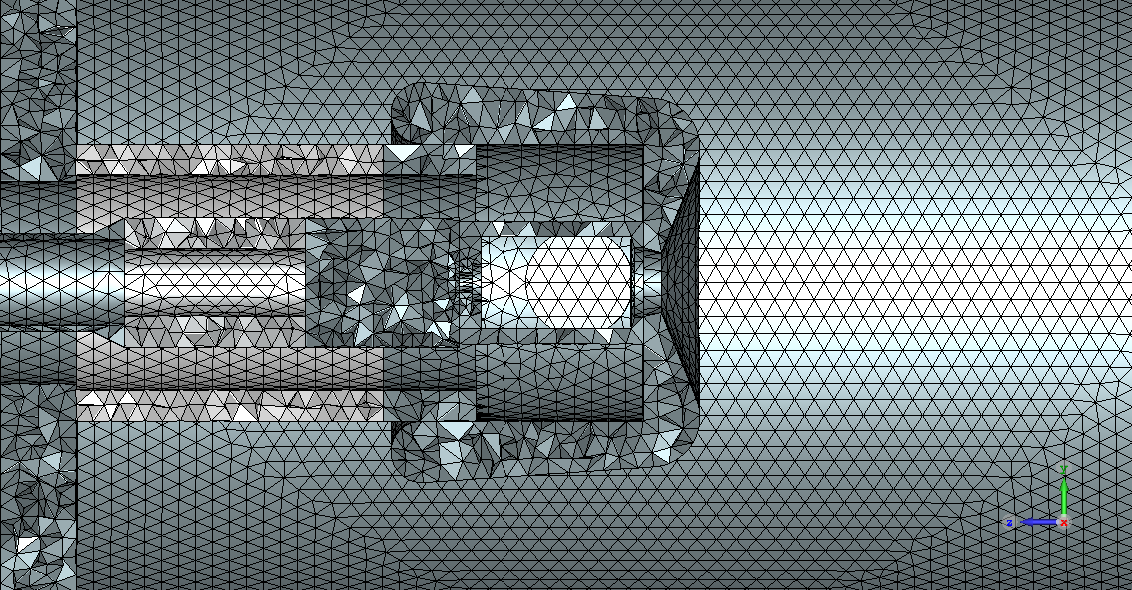
\includegraphics[width=\textwidth]{figures/200kV/cst/efield_orig_mesh}
   \end{subfigure}
   \begin{subfigure}{0.45\textwidth}
      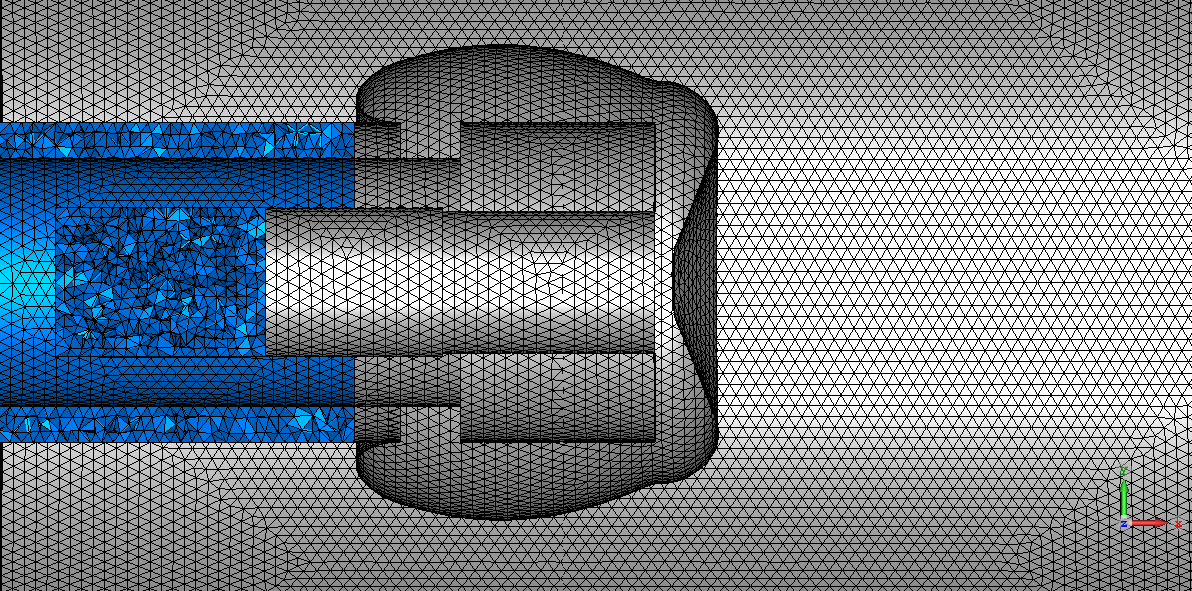
\includegraphics[width=\textwidth]{figures/200kV/cst/efield_mesh}
   \end{subfigure}
   \caption{Mesh of original and optimized geometry in CST.}
\end{figure}
\end{center}

\begin{center}
\begin{figure}[H]
   \begin{subfigure}{0.45\textwidth}
      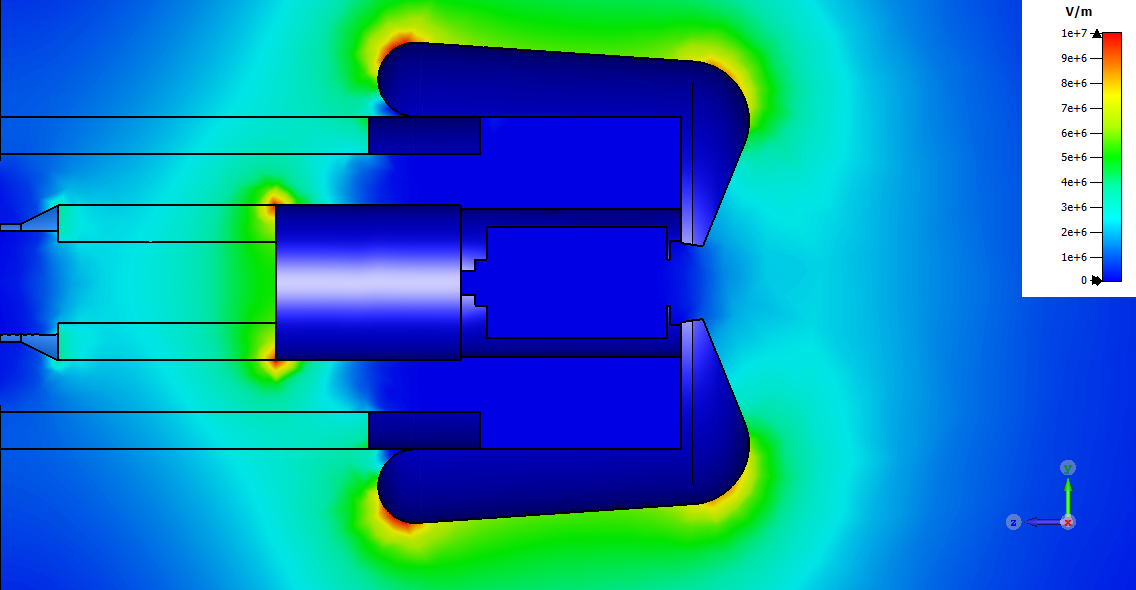
\includegraphics[width=\textwidth]{figures/200kV/cst/efield_orig}
   \end{subfigure}
   \begin{subfigure}{0.45\textwidth}
      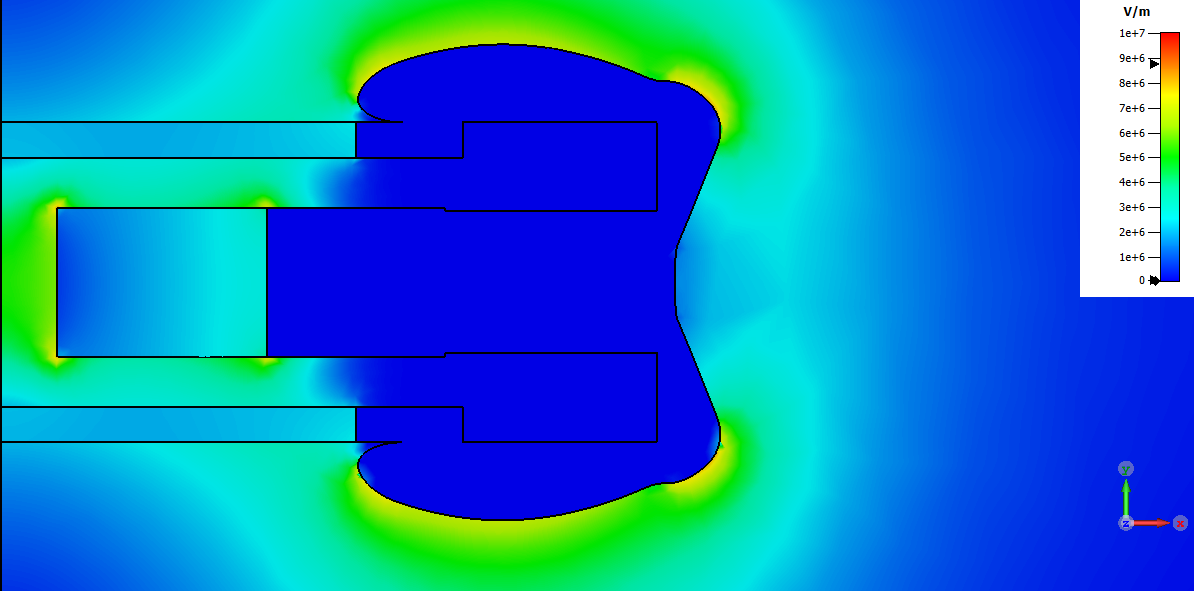
\includegraphics[width=\textwidth]{figures/200kV/cst/efield_insulator}
   \end{subfigure}
   \caption{Results of original and optimized geometry in CST.}
\end{figure}
\end{center}

\subsection{Astra}
In the future we may also optimize the electrode boundary next to the puck, i.~e.~patches 3, 4 and 5 to obtain optimal particle trajectories. The cost function will be computed using Astra.
The desired total bunch charge is $10$ pC with a beam current of $(20-100)\ \mu\mathrm{A}$, whereas a typical value would be $100$ fC. The bunch length is around $5$ ps with a normalized transversal emittance of $e_{x,y} \leq 1\ \mathrm{mm\ mrad}$. The desired energy resolution is $\frac{\Delta E}{E} \leq 10^{-4}$.
The tracking will be performed using individual bunches from a pulsed laser. The emission model may be derived from \cite{wagner}.


\clearpage
\phantomsection
\bibliographystyle{unsrt} %unsrt, abbrv, plain, acm
\bibliography{biblio}
\end{document}
